\documentclass[a4paper,10pt,DIV9, BCOR12mm, oneside,openright,openbib]{scrreprt}
	      %A4, 12mm Bindekorrektur Spiralbindung Sehnsucht-Design / 14mm Feldkamp
\usepackage[utf8]{inputenc}
\usepackage[T1]{fontenc}
\usepackage[ngerman]{babel}
\usepackage[fixlanguage]{babelbib}
\selectbiblanguage{german}
\usepackage{scrpage2}
\usepackage{tocloft}
\usepackage{graphicx}
\usepackage{wrapfig}
\usepackage{amsmath}
\usepackage{amssymb}
\usepackage{amsthm}
\usepackage{array}
\usepackage{tabularx}
\usepackage{tikz}
\usepackage{pdfpages}
\usepackage[german]{varioref}
\usepackage{makeidx}
\usepackage{listings}
\usepackage{textcomp}
\usepackage{hyperref}
\usepackage{caption}

\renewcommand*{\dictumwidth}{.4\textwidth}
\theoremstyle{definition}
\newtheorem{mydef}{Definition}[section]
\newtheorem{exmp}{Beispiel}[section]
\newtheorem{lemma}{Lemma}[section]
\theoremstyle{plain}
\newtheorem{mysat}{Satz}[section]
\makeindex
\begin{document}

%----------------------------
% Titelblatt
%----------------------------
\pagestyle{empty}
\begingroup
\centering
\vspace*{\baselineskip}

\rule{\textwidth}{1.6pt}\vspace*{-\baselineskip}\vspace*{2pt}
\rule{\textwidth}{0.4pt}\\[\baselineskip]

{\LARGE Skript\\[0.3\baselineskip] Mathematik \& Informatik } \\[0.5\baselineskip] 

\rule{\textwidth}{0.4pt}\vspace*{-\baselineskip}\vspace{3.2pt} 
\rule{\textwidth}{1.6pt}\\[\baselineskip]

\scshape 
Sammlung von Theoremen, Definitionen, Algorithmen, Code-Schnipseln und Strukturen \\ 
für die behandelten Themen in den Leistungskursen \\ Mathematik und Informatik\\[\baselineskip] 
Nottuln, 2013\par

\vspace*{3\baselineskip}

Autor\\[\baselineskip]
{\Large Alexander Pietz\par}
{\itshape Stand: \today \par}

\vfill 


\includegraphics[width=50px,height=51px]{../logo.png} \\[0.3\baselineskip]
{\large Hans-Böckler Berufskolleg\\ Münster}\par

\endgroup
%----------------------------
% /Titelblatt
%----------------------------
\newpage

\pagestyle{scrheadings}
\automark[section]{chapter}
\renewcommand{\headfont}{%
  \normalfont\sffamily
}
\ohead{\rightmark}
\chead{}
\ihead{\leftmark}
\ifoot{Mathematik \& Informatik Skript}
\ofoot{\pagemark}
\cfoot{}
\setheadtopline{1pt}
\setheadsepline{.2pt}
\setfootsepline{.4pt}


\tableofcontents
\listoffigures

\part{Mathematik}

\chapter{Analysis}

\section{Differenzialrechnung}
\subsection{Änderungsraten}
\subsection{Ableitungsfunktion}

\subsection{Kurvendiskussion}


\subsection{Gauß Algorithmus}

\section{Integralrechung}
Die Integralrechnung ist die Umkehrung der Differentiation und dient zur Berechnung von Flächen. Man unterscheidet zwischen unbestimmten und das bestimmten Integralen:

\subsection{Das bestimmte Integral}
Das bestimmte Integral einer Funktion ordnet dieser einen Zahlwert zu. Bildet man das bestimmte Integral einer reellen Funktion in einer Variablen, so lässt sich das Ergebnis im zweidimensionalen Koordinatensystem als Flächeninhalt der Fläche, die zwischen dem Graphen der Funktion, der x-Achse und den begrenzenden Parallelen zur y-Achse liegt, deuten. Hierbei zählen Flächenstücke unterhalb der x-Achse negativ. Man spricht vom orientierten Flächeninhalt. Diese Konvention wird gewählt, damit das bestimmte Integral eine lineare Abbildung ergibt, was sowohl für theoretische Überlegungen als auch für konkrete Berechnungen eine zentrale Eigenschaft des Integralbegriffs darstellt.

\subsection{Das unbestimmte Integral}
tbd

\chapter{Stochastik}
\dictum[Pierre Simon Marquis de Laplace]{Mit dem Wort "`Zufall"' gibt der Mensch nur seiner Unwissenheit Ausdruck.}
\section{Wahrscheinlichkeitsrechnung}
\subsection{Das Urnenexperiment}
Beim \textbf{Urnenexperiment} wird ein fiktives Gefäß, eine \textit{Urne}, mit einer Anzahl Kugeln gefüllt, welche anschließend zufällig gezogen werden. Damit ist gemeint, dass bei jedem Zug alle in der Urne befindlichen Kugeln die gleiche Wahrscheinlichkeit haben, ausgewählt zu werden (Laplace-Experiment). Dadurch kann die Bestimmung interessierender Wahrscheinlichkeiten auf die Lösung kombinatorischer Abzählprobleme zurückgeführt werden. Viele wichtige Wahrscheinlichkeitsverteilungen, wie beispielsweise die Binomialverteilung, können mit Hilfe von Urnenmodellen hergeleitet und veranschaulicht werden.
\begin{lemma}
 In der Urne befinden sich $n$ Kugeln, von denen $k$ gezogen werden.
\end{lemma}
Das Ziehen kann auf zwei verschiedene Arten erfolgen:
\begin{itemize}
 \item Eine Kugel wird gezogen und wieder zurückgelegt.
 \item Nach dem Ziehen der Kugel wird diese nicht wieder zurückgelegt.
\end{itemize}

\subsection{Abzählende Kombinatorik}
Die abzählende Kombinatorik ist ein Teilbereich der Kombinatorik, der sich mit der Bestimmung der Anzahl möglicher Anordnungen oder Auswahlen
\begin{itemize}
 \item unterscheidbarer oder nicht unterscheidbarer Objekte (d. h. „ohne“ bzw. „mit“ Wiederholung derselben Objekte) sowie
 \item mit oder ohne Beachtung ihrer Reihenfolge (d. h. „geordnet“ bzw. „ungeordnet“)
\end{itemize}
beschäftigt. In der modernen Kombinatorik werden diese Auswahlen oder Anordnungen auch als Abbildungen betrachtet, so dass sich die Aufgabe der Kombinatorik in diesem Zusammenhang im Wesentlichen darauf beschränken kann, diese Abbildungen zu zählen. Für das Rechnen mit Wahrscheinlichkeiten auf der Basis des Wahrscheinlichkeitsbegriffs von Laplace bildet die Kombinatorik eine wichtige Grundlage.\\
Ein verblüffendes Phänomen der Kombinatorik ist, dass sich oftmals wenige Objekte auf vielfältige Weise kombinieren lassen. Beim Zauberwürfel können beispielsweise die 26 Elemente auf rund 43 Trillionen Arten kombiniert werden. Dieses Phänomen wird oft als kombinatorische Explosion bezeichnet und ist auch die Ursache für das so genannte Geburtstagsparadoxon.\\
Alles in allem gibt es also zunächst einmal drei (oder auch nur zwei) verschiedene Fragestellungen, die ihrerseits noch einmal danach unterteilt werden, ob es unter den ausgewählten Elementen auch Wiederholungen gleicher Elemente geben darf oder nicht. Ist ersteres der Fall, spricht man von Kombinationen, Variationen oder Permutationen mit Wiederholung, andernfalls solchen ohne Wiederholung. Stellt man sich schließlich vor, dass die ausgewählten Elemente dabei einer Urne oder Ähnlichem entnommen werden, wird dementsprechend auch von Stichproben mit oder ohne Zurücklegen gesprochen:\\
{\small 
\begin{tabularx}{\columnwidth}{|X|X|X|}
\hline  & Ohne Wiederholung bzw. Zurücklegen & Mit Wiederholung bzw. Zurücklegen \\ 
\hline Mit Berücksichtigung der Reihenfolge
und k = n & Permutation ohne Wiederholung & Permutation mit Wiederholung \\ 
\hline Mit Berücksichtigung der Reihenfolge
und k $ < $ n & Variation ohne Wiederholung & Variation mit Wiederholung \\ 
\hline Ohne Berücksichtigung der Reihenfolge
und k $ < $ n & Kombination ohne Wiederholung & Kombination mit Wiederholung \\ 
\hline 
\end{tabularx}}

\subsubsection{Permutation}
\paragraph{Ohne Wiederholung}
Eine Permutation ohne Wiederholung ist eine Anordnung von n Objekten, die alle unterscheidbar sind. Nachdem es für das erste Objekt $ n $ Platzierungsmöglichkeiten gibt, kommen für das zweite Objekt nur noch $ n-1 $ Möglichkeiten in Betracht, für das dritte Objekt nur mehr $ n-2 $ und so weiter bis zum letzten Objekt, dem nur noch ein freier Platz bleibt. Die Anzahl der möglichen Permutationen von n Objekten wird demnach durch die Fakultät
\[ n! = n \cdot (n-1) \cdot \ldots \cdot 1 \]
angegeben.\\

\paragraph{Mit Wiederholung}
Eine Permutation mit Wiederholung ist eine Anordnung von $ n $ Objekten, von denen manche nicht unterscheidbar sind. Sind genau $ k $ Objekte identisch, dann sind diese auf ihren Plätzen vertauschbar, ohne dass sich dabei eine neue Reihenfolge ergibt. Auf diese Weise sind genau $ k! $ Anordnungen gleich. Die Anzahl der Permutationen von n Objekten, von denen $ k $ identisch sind, ist demnach durch
\[ \frac{n!}{k!} = n \cdot (n-1) \cdot \ldots \cdot (k+1) \]
gegeben.\\

\subsubsection{Variation}
\paragraph{Ohne Wiederholung}
Bei einer Variation ohne Wiederholung sollen $ k $ von $ n $ Objekten (mit $ k\leq n $) auf $ k $ verfügbare Plätze platziert werden, wobei jedes Objekt nur höchstens einen Platz einnehmen darf. Es gibt für den ersten Platz $ n $ mögliche Objekte, für den zweiten Platz $ n-1 $ Objekte usw. bis zum $ k $-ten Platz, für den es noch $ n-k+1 $ mögliche Objekte gibt. Insgesamt gibt es also
\[ n\cdot (n-1) \cdot \ldots \cdot (n-k+1) = \frac{n!}{(n-k)!} \]
mögliche Anordnungen.\\
\paragraph{Mit Wiederholung}
Bei einer Variation mit Wiederholung werden aus n Objekten $ k $ Objekte unter Beachtung der Reihenfolge ausgewählt, wobei Objekte auch mehrfach ausgewählt werden können. Nachdem jedes der $ n $ Objekte auf jedem der $ k $ Plätze der Auswahl erscheinen kann, gibt es demzufolge
\[ \underbrace{n \cdot \dotsc \cdot n}_{k\text{-mal}} = n^k \]
mögliche Anordnungen.

\subsubsection{Kombination}
\paragraph{Ohne Wiederholung}
Bei einer Kombination ohne Wiederholung geht man zunächst von einer Variation ohne Wiederholung aus, für die es bei $ k $ von $ n $ auszuwählenden Elementen$  \tfrac{n!}{(n-k)!} $ Möglichkeiten gibt. Nun aber können die $ k $ ausgewählten Elemente ihrerseits auf $ k! $ verschiedene Weisen angeordnet werden. Wenn diese verschiedenen Anordnungen allesamt keine Rolle spielen, also immer wieder als die gleiche Auswahl von Elementen gelten sollen, müssen wir das erhaltene Ergebnis noch einmal durch $ k! $ teilen und erhalten damit nur noch
\[ \frac{n!}{(n-k)! \, k!} = \frac{n (n-1)(n-2) \ldots (n-k+1)}{k!} = \binom{n}{n-k} = \binom{n}{k} \]
Möglichkeiten. Die Notation wird auch als \textit{Binomialkoeffizient} bezeichnet.
\paragraph{Mit Wiederholung}
Sollen aus einer Menge von $ n $ Elementen $ k $ Elemente ausgewählt werden, wobei ihre Reihenfolge weiterhin ohne Belang sein soll, sie sich aber nun auch wiederholen dürfen, wie das z. B. beim Ziehen mit Zurücklegen möglich ist, ergibt sich für die Zahl der Möglichkeiten folgende Formel :
\[ \frac{(n+k-1)!}{(n-1)! \, k!} = {n+k-1 \choose k} = {n+k-1 \choose n-1} \]

\subsubsection{Der Binomialkoeffizient}
Der \textbf{Binomialkoeffizient} ist eine mathematische Funktion, mit der sich eine der Grundaufgaben der Kombinatorik lösen lässt. Er gibt an, auf wie viele verschiedene Arten man k Objekte aus einer Menge von n verschiedenen Objekten auswählen kann (ohne Zurücklegen, ohne Beachtung der Reihenfolge). Der Binomialkoeffizient ist also die Anzahl der $k$-elementigen Teilmengen einer n-elementigen Menge.
\begin{exmp}
 "49 über 6" ist z. B. die Anzahl der möglichen Ziehungen beim Lotto (ohne Berücksichtigung der Zusatzzahl).
\end{exmp}

Ein Binomialkoeffizient hängt von zwei Zahlen $n$ und $k$ ab. Er wird mit dem Symbol  $ \binom nk $ geschrieben und als "n über k“, "k aus n“ oder "n tief k“ gesprochen. Die englische Abkürzung nCr für \textit{from n choose r} findet sich als Beschriftung auf Taschenrechnern und somit auch auf dem TI.\\


\begin{mydef}
Handelt es sich bei n um eine nichtnegative ganze Zahl mit $ n\geq k $, so kann man die aus der Kombinatorik bekannte Definition verwenden:
 \[ \binom nk = \frac{n!}{k! \cdot (n-k)!}. \]
 \[ \binom n0 = \binom nn = 1 \]
 \[ \binom n1 = \binom n{n-1} = n \]

\end{mydef}


\subsection{Zufallsgröße und Wahrscheinlichkeitsverteilung}
In der Stochastik ist eine \textbf{Zufallsgröße} eine Variable, deren Wert vom Zufall abhängig ist. Eine Zufallsgröße lässt sich formal als Funktion beschreiben, die den Ergebnissen eines Zufallsexperiments Werte (so genannte Realisierungen) zuordnet.\\
\\
Zufallsgröße $ X = X(\omega) $ sind funktional abhängig von einer den Zufall repräsentierenden Größe $ \omega $. Zum Beispiel kann $ \omega $ das zufällige Ergebnis eines Münzwurfs sein. Dann kann zum Beispiel eine Wette auf den Ausgang eines Münzwurfs mithilfe einer Zufallsgröße modelliert werden. Angenommen, es wurde auf Zahl gewettet, und wenn richtig gewettet wurde, wird 1 EUR ausgezahlt, sonst nichts. Sei X die Auszahlungssumme. Da der Wert von X vom Zufall abhängt, ist X eine Zufallsgröße. Sie bildet die Menge der Wurfergebnisse $ \{\text{Kopf}, \text{Zahl}\} $ auf die Menge der möglichen Auszahlungsbeträge $ \{0, 1\} $ ab:
\[  X(\omega) = \begin{cases} 0, & \text{wenn }\omega = \text{Kopf},\\ 1, & \text{wenn }\omega = \text{Zahl}. \end{cases}  \]
Wettet man bei zwei Münzwürfen beide Male auf Kopf und bezeichnet die Kombination der Ausgänge der Münzwürfe mit $ \omega=\left(\omega_1,\omega_2\right) $, so lassen sich beispielsweise folgende Zufallsgrößen untersuchen:
\begin{itemize}
\item $ X_1(\omega) := X(\omega_1) \in\{0,1\} $ als Auszahlung nach der ersten Wette,\\
\item $ X_2(\omega) := X(\omega_2) \in\{0,1\} $ als Auszahlung nach der zweiten Wette,\\
\item $ S(\omega) := X(\omega_1) + X(\omega_2) \in\{0,1,2\} $ als Summe der beiden Auszahlungen.\\
\end{itemize}
Zufallsgrößen selbst werden üblicherweise mit einem Großbuchstaben bezeichnet (hier $ X_1, X_2, S $), während man für die Realisierungen die entsprechenden Kleinbuchstaben verwendet (so beispielsweise für $ \omega=\left(\text{Zahl},\text{Kopf}\right) $ die Realisierungen $ x_1 = 1, x_2=0, s=1 $).\\
Im Beispiel hat die Menge $ \Omega = \{\text{Kopf}, \text{Zahl}\} $ eine konkrete Interpretation. In der weiteren Entwicklung der Wahrscheinlichkeitstheorie ist es oft zweckmäßig, die Elemente von $ \Omega $ als abstrakte Repräsentanten des Zufalls zu betrachten, ohne ihnen eine konkrete Bedeutung zuzuweisen, und dann sämtliche zu modellierende Zufallsvorgänge als Zufallsgröße zu erfassen.\\

\subsubsection{Erwartungswert}
\begin{mydef}
Eine Zufallsgröße $X$ nehme die Werte $ a_1, a_2, .. , a_m  $ mit den Wahrscheinlichkeiten $ P(X=a_1), P(X=a_2), ... P(X=a_m) $ an. Dann wird der zu erwartende Mittelwert $ E(X) $ der Verteilung als \textit{Erwartungswert der Zufallsgröße X} bezeichnet. Es gilt:
\[ \mu = \operatorname{E}(X)=\sum_{i=1}^m a_i * P(X=a_i)  \]
\end{mydef}

\subsubsection{Varianz}
\begin{mydef}
Gegeben sei ein quantitatives Merkmal mit den Merkmalsausprägungen $ x_1, x_2, .., x_m $ und den zugehörigen relativen Häufigkeiten $ h(x_1), h(x_2), .., h(x_m) $. Dann gilt für die Varianz:
\[ s^2=(\sum_{i=1}^m x_i^2 * h(x_i))- \mu^2  \]
\end{mydef}

\subsection{Satz von Bayes}
Sei $A$ ein Ereignis, das uns interessiert, und $B$ eine Bedingung, unter der wir das Ereignis betrachten. Dann gilt:
\begin{mydef}
\textit{Die Wahrscheinlichkeit $ P_{B}(A) $ für A unter der Bedingung B} berechnet sich wie folgt: 
\[ P_{B}(A) = \frac{P(A \cap{B})}{P(B)} \] 
\end{mydef}

\subsubsection{Mehrfeldtafel}
\textbf{Mehrfeldtafeln} sind Tabellen, die die absoluten oder relativen Häufigkeiten von Kombinationen bestimmter Merkmalsausprägungen enthalten. Kontingenz hat dabei die Bedeutung des \underline{gemeinsamen Auftretens} von zwei Merkmalen. Das bedeutet, es werden Häufigkeiten für mehrere miteinander durch 'und' oder 'sowie' verknüpfte Merkmale dargestellt. Diese Häufigkeiten werden ergänzt durch deren Randsummen, die die sogenannten \textbf{Randhäufigkeiten} bilden.\\ 

\subsubsection{Vierfeldertafel}
Unter einer \textbf{Vierfeldertafel} versteht man eine vereinfachte Kontingenztafel , die Zahlenwerte der möglichen Ergebnisse eines durchgeführten Tests auf einen Blick präsentiert. \\ 
Die Vierfeldtafel bildet sich nach dem \textit{Satz von Bayes} wie folgt: \\ 
\begin{center}
\begin{tabular}{|c|c|c|c|}
\hline Merkmal & A &$   \bar{A}  $ & Summe \\ 
\hline B &$   P({A}\cap{B}) $  &$   P({\bar{A}}\cap{B})  $ &$  P(B) $ \\ 
\hline  $ \bar{B} $  & $ P({A}\cap{\bar{B}}) $ & $  P({\bar{A}}\cap{\bar{B}}) $ & $ P({\bar{B}}) $  \\ 
\hline Summe & $ p(A) $ & $ P({\bar{A}}) $ & 1 \\ 
\hline 
\end{tabular}
\end{center}

\subsubsection{Stochastische Unabhängigkeit}
\textbf{Stochastische Unabhängigkeit} ist ein Konzept, welches die Vorstellung von sich \underline{nicht gegenseitig beeinflussenden} Zufallsereignissen formalisiert. Sind zwei Ereignisse stochastisch unabhängig, dann ändert sich die Wahrscheinlichkeit dafür, \textit{dass das eine eintritt, nicht, wenn das andere eintritt} (beziehungsweise nicht eintritt). \\ 
Insbesondere Ereignisse, die mit positiver Wahrscheinlichkeit eintreten und sich gegenseitig ausschließen oder bedingen, sind voneinander abhängig. Dass Ereignisse sich gegenseitig ausschließen, wird häufig mit deren Unabhängigkeit verwechselt.\\ 
\linebreak
Stehen die Wahrscheinlichkeiten in den Spalten oder in den Zeilen einer \underline{Vierfeldertafel} im gleichen festen Zahlenverhältnis, dann sind die zugehörigen Merkmale voneinander unabhängig; sonst sind sie voneinander abhängig. \\
\linebreak
Gilt für zwei Ereignisse A,B, dass $ P({A}\cap{B})= P(A) * P(B) $, d.h. also dass $ P(B) = P_{A}(B)$, dann nennt man A,B \textbf{stochastisch voneinander unabhängig}, sonst  \textbf{stochastisch voneinander abhängig}.
\paragraph{Sensitivität}
Die Sensitivität (auch Richtig-Positiv-Rate, Empfindlichkeit oder Trefferquote) gibt den Anteil der korrekt als positiv klassifizierten Objekte an der Gesamtheit der tatsächlich positiven Objekte an. Beispielsweise entspricht Sensitivität bei einer medizinischen Diagnose dem Anteil an tatsächlich Kranken, bei denen die Krankheit auch erkannt wurde.
\paragraph{Spezifität}
Die Spezifität (auch Richtig-Negativ-Rate oder kennzeichnende Eigenschaft) gibt den Anteil der korrekt als negativ klassifizierten Objekte an der Gesamtheit der in Wirklichkeit negativen Objekte an. Beispielsweise gibt die Spezifität bei einer medizinischen Diagnose den Anteil der Gesunden an, bei denen auch festgestellt wurde, dass keine Krankheit vorliegt.
\paragraph{Umkehrung des Baumdiagramms}
Vertauscht man die Reihenfolge der betrachteten Merkmale bei einem Baumdiagramm, dann erhält man das so genannte \textbf{umgekehrte Baumdiagramm}. Die Wahrscheinlichkeiten, die an den einzelnen Pfaden stehen, unterscheiden sich im Allgemeinem bei einem Baumdiagramm und seiner Umkehrung, denn sie beziehen sich auf verschiedene Merkmale und daher auf verschiedene Teilgesamtheiten. \\
Dagegen stimmen die Pfadwahrscheinlichkeiten bis auf die Reihenfolge überein, da sie die Wahrscheinlichkeiten der inneren Felder derselben Vierfeldtafel sind.
\paragraph{Allgemeine Multiplikationsregel}
$ A_{1}, A_{2}, ..., A_{3} $ sind Ereignisse einer Ergebnismenge S. Dann gilt: \\
\[ P(A_{1} \cap A_{2} \cap ... \cap A_{K}) = P(A_{1}) * P_{A_{1}}(A_{2}) * P_{A_{1} \cap A_{2} }(A_{2}) * ... * P_{A_{1} \cap A_{2} \cap ... \cap A_{k}}(A_{2})\]
\paragraph{Satz der totalen Wahrscheinlichkeit}
Fasst man gleiche Pfad-Enden zusammen, so gilt für die neue Pfadwahrscheinlichkeit:
\[ P(B) = P(A \cap B) + P(\bar{A} \cap B) = P(A) * P_{A}(B) + P(\bar{A})  * P_{\bar{A}}(B) \]

Aus der Summe von Produkten lässt sich ablesen, wie sich das Ergebnis B "zusammensetzt" (ein Pfad über das Ereignis $ A $, ein Pfad über das Ereignis $ \bar{A} $) \\
Allgemein erhält man analog:
\[ P(B) = P(A_{1}) * P_{A_{1}}(B) + P(A_{2}) * P_{A_{2}}(B) + ... + P(A_{n}) * P_{A_{n}}(B) = \displaystyle\sum_{i=1}^n P(A_{i}) * P_{A_{i}}(B) \]

\subsection{Die Binomialverteilung}
Die Binomialverteilung ist eine der wichtigsten diskreten Wahrscheinlichkeitsverteilungen.\\
\\
Sie beschreibt die Anzahl der Erfolge in einer Serie von gleichartigen und unabhängigen Versuchen, die jeweils genau zwei mögliche Ergebnisse haben ("Erfolg“ oder "Misserfolg“). Solche Versuchs-Serien werden auch Bernoulli-Prozesse genannt.\\
\\
Ist $ p $ die Erfolgswahrscheinlichkeit bei einem Versuch und die Anzahl der Versuche $ n $, dann bezeichnet man mit $ B_{n,p}(k) $ die Wahrscheinlichkeit, genau $ k $ Erfolge zu erzielen.\\
\\
Die Binomialverteilung und der Bernoulli-Versuch können mit Hilfe des Galtonbretts veranschaulicht werden. Dabei handelt es sich um eine mechanische Apparatur, in die man $ n $ Kugeln wirft. Diese fallen dann zufällig in eines von mehreren Fächern, wobei die Aufteilung der Binomialverteilung entspricht. Je nach Konstruktion sind unterschiedliche Parameter $ p $ möglich.\\
\subsubsection{Eigenschaften}
\paragraph{Definition}
Die Wahrscheinlichkeitsverteilung mit der Wahrscheinlichkeitsfunktion
\[  B_{n,p}(k) = \binom nk p^k (1-p)^{n-k} bei k=0,1,\dotsc, n \]
heißt die \textbf{Binomialverteilung} zu den Parametern $ n $ (Anzahl der Versuche) und $ p\in [0,1] $ (der Erfolgs- oder Trefferwahrscheinlichkeit).\\

\subparagraph{Symmetrie}
Die Binomialverteilung ist in den Spezialfällen $ p = 0, p = 0{,}5 $ und $ p = 1 $ symmetrisch und ansonsten asymmetrisch.
\subparagraph{Erwartungswert}
Die Binomialverteilung besitzt den Erwartungswert $ n*p $.
\subparagraph{Varianz}
Die Binomialverteilung besitzt die Varianz $ n*p*(1-p) $.

\subsubsection{Sigma - Umgebungen}
Der Abstand vom Erwartungswert zur x-Koordinate eines Wendepunkts heißt Standardabweichung und wird mit $ \sigma $ (lies: sigma) bezeichnet.
Mit Mitteln der Analysis kann $ \sigma = \sqrt{n*p*(1-p)} $
bestimmt werden.\\
\\
Für $ n $-stufige Bernoulli-Versuche gilt under der sog. Laplace-Bedingung $ \sigma > 3 $:\\
Die Wahrscheinlichkeit, dass die Anzahl der Treffer in der 2 $ \sigma $-Umgebung des Erwartungswerts liegt, beträgt ca. $ 0,954 $, für die  3 $ \sigma $-Umgebung sind es ca. $ 0,997 $

\subsubsection{Standardisierung einer Zufallsgröße}
Eine Zufallsgröße mit dem Erwartungswert 0 und der Varianz 1 heißt standardisiert. Jede Zufallsgröße lässt sich mit Hilfe der Transformation standardisieren:
\begin{enumerate}
 \item Die Höhen der Rechtecke in der Histogrammdarstellung müssen mit dem Faktor $ \sigma $ multipliziert werden, da die Rechtecksbreiten um den Faktor $ 1/\sigma $ verändert werden.\\
 \item Durch die Standardisierung wir bei der Verteilungsfunktion nur die Lage der Sprungstellen, nicht deren Höhe verändert. 
\end{enumerate}
\subsubsection{Die Normalverteilung}
Die Bedeutung der Normalverteilung beruht unter anderem auf dem zentralen Grenzwertsatz, der besagt, dass eine Summe von $ n $ unabhängigen, identisch verteilten Zufallsvariablen mit endlicher Varianz im Grenzwert $ n\rightarrow\infty $ normalverteilt ist. Das bedeutet, dass man Zufallsvariablen dann als normalverteilt ansehen kann, wenn sie durch Überlagerung einer großen Zahl von unabhängigen Einflüssen entstehen, wobei jede einzelne Einflussgröße einen im Verhältnis zur Gesamtsumme unbedeutenden Beitrag liefert.\\
Die Standardabweichung $ \sigma $ beschreibt die Breite der Normalverteilung und hängt mit der Halbwertsbreite zusammen. Es gilt näherungsweise:\\
\\
Im Intervall der Abweichung $ \pm \sigma  $vom Mittelwert sind  68,27 \% aller Messwerte zu finden,\\
Im Intervall der Abweichung $ \pm 2\sigma $ vom Mittelwert sind 95,45 \% aller Messwerte zu finden,\\
Im Intervall der Abweichung $ \pm 3\sigma $ vom Mittelwert sind 99,73 \% aller Messwerte zu finden.\\\\
\\
Und ebenso lassen sich umgekehrt für gegebene Wahrscheinlichkeiten die maximalen Abweichungen vom Mittelwert finden:\\
\\
50 \% aller Messwerte haben eine Abweichung von höchstens $ 0{,}675\sigma $ vom Mittelwert,\\
90 \% aller Messwerte haben eine Abweichung von höchstens $ 1{,}645\sigma $ vom Mittelwert,\\
95 \% aller Messwerte haben eine Abweichung von höchstens $ 1{,}960\sigma $ vom Mittelwert,\\
99 \% aller Messwerte haben eine Abweichung von höchstens $ 2{,}576\sigma $ vom Mittelwert.\\
\\\\
Die \textbf{Dichtefunktion} der Standardnormalverteilung ist
\[  \varphi(x)=\frac{1}{\sqrt{2\pi}} e^{-\frac{1}{2} x^2}\ \]
\subsubsection{Das Bernoulli-Experiment}
Zufallsgrößen mit einer \textbf{Bernoulli-Verteilung} benutzt man zur Beschreibung von zufälligen Ereignissen, bei denen es nur zwei mögliche Versuchsausgänge gibt. Einer der Versuchsausgänge wird meistens mit Erfolg bezeichnet und der komplementäre Versuchsausgang mit Misserfolg. Die zugehörige Wahrscheinlichkeit p für einen Erfolg nennt man Erfolgswahrscheinlichkeit und $ q=1-p $ die Wahrscheinlichkeit eines Misserfolgs. Beispiele:
\begin{list}{}{}
\item Werfen einer Münze: Kopf (Erfolg), $ p=1/2 $, und Zahl (Misserfolg), $ q=1/2 $. \\
\item Werfen eines Würfels, wobei nur eine “6“ als Erfolg gewertet wird: $ p=1/6 $, $ q=5/6 $.\\
\item Qualitätsprüfung (einwandfrei, nicht einwandfrei).\\
\end{list}
\paragraph{Erwartungswert}
Die Bernoulli-Verteilung mit Parameter p hat den Erwartungswert:
\[\operatorname{E}\left(X\right)=p\]
\paragraph{Varianz}
Die Bernoulli-Verteilung besitzt die Varianz:
\[\operatorname{Var}(X) = p(1-p)= pq \], denn: \[ \operatorname{E}\left(X^2\right)-\operatorname{E}(X)^2=p-p^2 = p\cdot(1-p) = pq\]
\paragraph{Beziehung zur Binomialverteilung}
Die Bernoulli-Verteilung ist ein Spezialfall der Binomialverteilung für $ n=1 $. Mit anderen Worten, die Summe von unabhängigen Bernoulli-verteilten Zufallsgrößen mit identischem Parameter p genügt der Binomialverteilung. Die Binomialverteilung ist die n-fache Faltung der Bernoulli-Verteilung mit gleicher Wahrscheinlichkeit ,$ p $.

\subsubsection{Die Bernoulli-Kette}
Eine \textbf{Bernoulli-Kette} ist ein zeitlich diskreter stochastischer Prozess, der aus einer endlichen oder abzählbar-unendlichen Folge von unabhängigen Versuchen mit Bernoulli-Verteilung besteht, das heißt, für jeden der Zeitpunkte 1, 2, 3, … wird “ausgewürfelt“, ob ein Ereignis mit Wahrscheinlichkeit $ p $ eintritt, oder nicht.\\
Der Prozess kann durch eine Folge von Zufallsvariablen $ X_1, X_2, X_3 $,..., beschrieben werden, von denen jede mit der konstanten Wahrscheinlichkeit p den Wert $ X=1 $ (Erfolg) und mit der Wahrscheinlichkeit $ q=1-p $ den Wert $ X=0 $ (Misserfolg) annimmt. \\
Die Anzahl $ k $ erfolgreicher Versuche nach Durchführung von insgesamt $ n $ Versuchen; sie folgt einer Binomialverteilung.\\
 \begin{exmp}
   Ein betrunkener Fußgänger  bewegt sich bei jedem Schritt mit der Wahrscheinlichkeit $ p $ vorwärts, mit der Wahrscheinlichkeit $ q $ rückwärts. Man interessiert sich für die Entfernung vom Ausgangspunkt $ 2k-n $. Ein solches Modell wird in der Physik als eindimensionale Zufallsbewegung (Random Walk) bezeichnet.\\
 \end{exmp}
Die Zufallsvariable $ k $, die angibt, wie viele von $ n $ Bernoulli-Versuchen erfolgreich waren, folgt der Binomialverteilung. Wir leiten diese Verteilung anhand eines Beispiels her:\\
\\
Beim Würfeln werde die Sechs als Erfolg gewertet; die Erfolgswahrscheinlichkeit ist also $ p=1/6 $, die komplementäre Misserfolgswahrscheinlichkeit $ q=5/6 $. Gefragt sei nun nach der Wahrscheinlichkeit, in $ n=5 $ Würfen genau $ k=2 $ Sechsen zu werfen.\\
\\
Antwort: Die Wahrscheinlichkeit, erst zwei Sechsen, dann drei Nicht-Sechsen zu werfen, ist $ p^2q^3 $. Da es auf die Reihenfolge aber nicht ankommt, ist diese Wahrscheinlichkeit zu multiplizieren mit der Anzahl der Möglichkeiten, zwei (ununterscheidbare) Sechserwürfe auf fünf Würfe zu verteilen. Der Kombinatorik zufolge ist diese Anzahl durch den Binomialkoeffizienten “5 über 2“ gegeben; die gesuchte Wahrscheinlichkeit lautet also:\\
 \[ B(2 |p,5) = \left( \begin{matrix} 5\\ 2 \end{matrix} \right) p^2 q^{5-2}. \]
Davon verallgemeinert, lautet die Wahrscheinlichkeit, in n Bernoulli-Versuchen genau k mal Erfolg zu haben,\\
 \[ B(k|p,n) = \left( \begin{matrix} n\\ k \end{matrix} \right) p^k q^{n-k} \]
mit $ q=1-p $. Diese Funktion heißt \textbf{Binomialverteilung}.


\subsubsection{Das Histogramm}
Ein \textbf{Histogramm} ist eine graphische Darstellung der Häufigkeitsverteilung metrisch skalierter Merkmale. Es erfordert die Einteilung der Daten in Klassen, die eine konstante oder variable Breite haben können. Bei Bernulli-Versuchen bietet sich zunächst eine konstante Breite von 1 an. Es werden direkt nebeneinander liegende Rechtecke von der Breite der jeweiligen Klasse gezeichnet, deren Flächeninhalte die (relativen oder absoluten) Klassenhäufigkeiten darstellen. Die Höhe jedes Rechtecks stellt dann die (relative oder absolute) Häufigkeitsdichte dar, also die (relative oder absolute) Häufigkeit dividiert durch die Breite der entsprechenden Klasse.

\section{Beurteilende Statistik}
In der Beurteilenden Statistik versucht man, aus den bei mehrmaligen Durchführungen eines Zufallsexperimentes aufgetretenen Ergebnissen auf die unbekannte, dem Zufallsexperiment tatsächlich zugrundeliegende Wahrscheinlichkeitsverteilung zu schließen.

\subsection{Hypothesentest}
 Das Testen von Hypothesen ist immer ein Vorgang, den man in mehrere Schritte unterteilen kann:

  \begin{enumerate}
    \item Formulierung der Nullhypothese $H_{0}$ und der Alternativhypothese $H_{1}$
    \item Festlegung des Signifikanzniveaus
    \item Bestimmung des Annahme- und Ablehnungsbereichs der Nullhypothese
    \item Ziehung der Stichprobe
    \item Treffen der Testentscheidung und Interpretation:
    \item Liegt das Ergebnis der Stichprobe innerhalb des Annahmebereichs, wird $H_{0}$ angenommen, anderenfalls abgelehnt
  \end{enumerate}

  Für das Aufstellen der Hypothesen gilt:
  \begin{itemize}
    \item Was ich zeigen oder beweisen will, gehört in die Alternativhypothese
    \item Das Gleichheitszeichen gehört immer in die Nullhypothese
    \item Beim aufstellen der Nullhypothese geht man davon aus, ``Alles bleibt beim alten, nichts hat sich geändert''
  \end{itemize}

%-> http://lehrerfortbildung-bw.de/faecher/mathematik/gym/fb2/modul4/2_higru/2_hypo/02_beurteilende_statistik_testen_von_hypothesen.pdf



\chapter{Zahlentheorie}
\dictum[Werner Fuld]{Mathematiker sind Betriebsunfälle der Natur.}
Hinweis \footnote{Teilweise entnommen aus \cite{Bouw2010} und \cite{Maier2009/10}}
\section{Teilbarkeit}
\begin{mydef} \label{Teilbark} \index{Teilbarkeit}
Eine ganze Zahl $b$ heißt durch eine ganze Zahl $a \neq 0$ teilbar, falls es ein $x \in \mathbb{Z}$ gibt, so dass $b = ax$ ist, und wir schreiben $ a \mid b$. Man nennt $a$ einen \underline{Teiler} von $b$ ,und $b$ heißt \underline{Vielfaches} von $a$. Falls $b$ nicht durch $a$ teilbar ist, schreiben wir $a \nmid b$
\end{mydef}

\section{Kongruenzen}\index{Kongruenz} In diesem Kapitel studieren wir die Theorie der Kongruenzen. Kongruenzen beschreiben Teilbarkeitsrelationen. Man findet sie auch im täglichen Leben: Uhren geben die Stunden entweder modulo 12 oder modulo 24 an. Die Wochentage rechnen wir modulo 7 und die Monate modulo 12. Sobald wir die richtigen Werkzeuge bereit gestellt haben, können wir genauso gut mit Kongruenzen rechnen wie mit Gleichungen.

\begin{mydef} Sei m eine natürliche Zahl und seien $a, b$ ganze Zahlen. Wir sagen, dass $a$ kongruent zu $b$ modulo $m$ ist, falls $m \mid (b-a)$. (Äquivalent: es existiert ein $k \in Z$ mit $b = a + km$.) Wir schreiben: $a \equiv\ b$ (mod $m$). Die Zahl $m$ heißt der Modul der Kongruenz. Zum Beispiel ist $200 \equiv 11$ (mod $9$), da $9$ ein Teiler von $200-11=189$ ist. Anders formuliert: $200$ und $11$ haben den gleichen Rest nach Division durch $9$, nämlich $2$.
\end{mydef}
\begin{mysat} Kongruenz ist eine Äquivalenzrelation, d.h. es gelten die folgenden Eigenschaften:
\paragraph{Reflexivität}\index{Reflexivität} $a \equiv a$ (mod $m$), für alle $a \in Z$,
\paragraph{Symmetrie}\index{Symmetrie} Falls $a \equiv b$ (mod $m$), so gilt auch $b \equiv a$ (mod $m$),
\paragraph{Transitivität}\index{Transitivität} Falls $a \equiv b$ (mod $m$) und $b \equiv c$ (mod $m$), so gilt auch $a \equiv c$ (mod m).
\end{mysat}

\section{Nullteiler}\index{Nullteiler}
In der \textit{abstrakten Algebra} ist ein Nullteiler eines Ringes $R$ ein vom Nullelement $0$\index{Nullelement} verschiedenes Element $a$, für das es ein vom Nullelement $0$ verschiedenes Element $b$ gibt, so dass $ab = 0$.

\section{Größter gemeinsamer Teiler}
\begin{mydef}
Der $\operatorname{ggT}$ zweier ganzer Zahlen $a$ und $b$ ist eine ganze Zahl m mit der Eigenschaft, dass sie Teiler sowohl von $a$ als auch von $b$ ist und dass jede ganze Zahl, die ebenfalls die Zahlen $a$ und $b$ teilt, ihrerseits Teiler von $m$ ist. 
\end{mydef}

\section{Kleinstes gemeinsames Vielfaches}
\begin{mydef}
Das \textit{kleinste gemeinsame Vielfache} zweier ganzer Zahlen $m$ und $n$ ist die kleinste natürliche Zahl, die sowohl Vielfaches von $m$ als auch Vielfaches von $n$ ist.
\end{mydef}

\section{Euklidscher Algorithmus}
Der \textbf{erweiterte euklidische Algorithmus} berechnet neben dem größten gemeinsamen Teiler $\operatorname{ggT}(a,b)$ zweier natürlicher Zahlen $a$ und $b$ noch zwei ganze Zahlen $s$ und $t$, die die folgende Gleichung erfüllen:
\[\operatorname{ggT}(a,b) = s \cdot a + t \cdot b \]
Das Haupteinsatzgebiet des erweiterten euklidischen Algorithmus ist die Berechnung der \textbf{inversen Elemente in ganzzahligen Restklassenringen}, denn wenn der Algorithmus das Tripel $(d=\operatorname{ggT}(a,b), s, t)$ ermittelt, ist entweder $d=1$ und damit $1\equiv t\cdot b \pmod a$, $t$ also das \textit{multiplikative Inverse} von $b$ modulo $a$, oder aber $d\neq 1$, was bedeutet, dass $b$ modulo $a$ kein Inverses hat.

\section{Primfaktorzerlegung}
Die Primfaktorzerlegung ist die Darstellung einer natürlichen Zahl $n$ als Produkt aus Primzahlen, die dann als Primfaktoren von $n$ bezeichnet werden.
\begin{mydef}
Sei $n$ eine natürliche Zahl. Eine Zahl $p$ heißt Primfaktor von $n$,
\begin{itemize}
 \item wenn $p$ ein Teiler von n ist und 
 \item $p$ eine Primzahl ist.
\end{itemize}
Die Primfaktorzerlegung ist die Darstellung der Zahl $n$ als Produkt ihrer Primfaktoren. Da die Multiplikation kommutativ und assoziativ ist, ist die Reihenfolge der Primfaktoren aus Sicht der Zahlentheorie unwichtig. Die Primfaktorzerlegung der Eins kann als leeres Produkt betrachtet werden. Wenn $n$ selbst eine Primzahl ist, so ist sie selbst ihr einziger Primfaktor. Gibt es mehr als einen Primfaktor, so wird n zusammengesetzte Zahl genannt. Die Null ist niemals Teil der multiplikativen Gruppe und wird von solchen Betrachtungen ausgeschlossen.\\
Mehrfach auftretende Primfaktoren können mittels Exponenten-Schreibweise zusammengefasst werden.
\end{mydef}

\section{Satz von Euler-Fermat}
\[a^{\varphi(n)} \equiv 1\pmod{n}\]
\subsection{Kleiner fermatscher Satz}
\[a^p \equiv a\pmod{p}\]
Ist $a$ kein Vielfaches von $p$ gilt:
\[a^{p-1} \equiv 1\pmod{p} \]

\section{Eulersche Phi-Funktion}
Die eulersche Phi-Funktion ist eine zahlentheoretische Funktion. Sie gibt für jede natürliche Zahl $n$ an, wie viele zu $n$ teilerfremde natürliche Zahlen es gibt, die nicht größer als $n$ sind:
\[ \varphi(n) \colon= \Big| \{a \in \mathbb{N} \mid 1 \leq a \leq n \wedge \operatorname{ggT}(a,n) = 1 \} \Big| \]

\subsection{Eigenschaften und Berechnung}
Allgemein lässt sich der Wert der eulerschen Phi-Funktion aus der Primfaktorzerlegung berechnen:
\paragraph{Multiplikative Funktion}
Für teilerfremde Zahlen m und n gilt:
\[\varphi (m \cdot n) = \varphi (m) \cdot \varphi (n) \]
\paragraph{Berechnung für Primzahlen}
Da eine Primzahl $p$ nur durch 1 und sich selbst teilbar ist, ist sie zu den Zahlen 1 bis $p - 1$ teilerfremd. Weil sie größer als 1 ist, ist sie außerdem \textit{nicht} zu sich selbst teilerfremd. Es gilt daher
\[\varphi(p) = p-1. \]

\section{Gruppen, Ringe, Körper}
Siehe hierzu bitte Anhang \vref{subsec:GRK}.


\chapter{Lineare Algebra / Analytische Geometrie} 
\dictum[René Descartes]{Jedes Problem, das ich gelöst hatte, wurde zu einer Regel, mit deren Hilfe später weitere Probleme gelöst werden konnten.}
 \section{Matrizenrechnung}
Eine Matrix ist ein rechteckiges Schema, dessen Elemente üblicherweise Zahlen, aber auch andere mathematische Elemente wie Variablen oder Funktionen sein können. Sie besteht aus $m$ Zeilen und $n$ Spalten. Matrizen können beliebige Dimensionalität besitzen.
\subsection{Notation}
Eine \textbf{Matrix} A vom Typ $(m,n)$ mit Zahlen, die in $m$ Zeilen und $n$ Spalten angeordnet sind:
\[A_{m,n} =
 \begin{pmatrix}
  a_{1,1} & a_{1,2} & \cdots & a_{1,n} \\
  a_{2,1} & a_{2,2} & \cdots & a_{2,n} \\
  \vdots  & \vdots  & \ddots & \vdots  \\
  a_{m,1} & a_{m,2} & \cdots & a_{m,n}
 \end{pmatrix}\]
 Man schreibt: $A_{m,n} = (a_{i,k})_{m,n} $ mit $i= 1,2,..,m$ und $k= 1,2,..,n$.
\\[5ex]
 Matrizen, die aus lauter Nullen bestehen, nennt man \textbf{Nullmatrix}. Man schreibt dafür auch O.
\[ O_{mn} = \begin{pmatrix} 0 & \cdots & 0 \\ \vdots & \ddots & \vdots \\ 0 & \cdots & 0 \end{pmatrix}.\]
\subsection{Matrizenaddition}
Zwei Matrizen können addiert werden, wenn sie vom selben Typ sind, das heißt, wenn sie dieselbe Anzahl von Zeilen und dieselbe Anzahl von Spalten besitzen. 
Seien $A$ und $B$ Matrizen über einer Menge $R$, dessen abelsche Gruppe ein Ring ist.\footnote{lt. Ringtheorie Voraussetzung zur Addition von Matrizen\cite{Artin1998}}. Jedes Element der Summenmatrix ist die Summe der Elemente der Matrizen $A$ und $B$: 
\[ A + B = ( a_{ij} + b_{ij} ) = \begin{pmatrix} a_{11} + b_{11} & \cdots & a_{1n} + b_{1n} \\ \vdots & \ddots & \vdots \\ a_{m1} + b_{m1} & \cdots & a_{mn} + b_{mn} \end{pmatrix} \]
\\[5ex]
\subsubsection{Die Einheitsmatrix}
Die Einheitsmatrix ist eine quadratische Matrix, auf der alle Elemente den Wert Null haben, bis auf die Elemente, die auf der Diagonale (von links oben nach unten rechts) liegen und den Wert Eins haben. 
\[I_n = \begin{pmatrix} 1 & 0 & \cdots & 0 \\ 0 & 1 & \ddots & \vdots \\ \vdots & \ddots & \ddots & 0 \\ 0 & \cdots & 0 & 1 \end{pmatrix}\]
\begin{small}Beachte, dass $0$ das Nullelement und $1$ das Einselement des jeweiligen Ringes, über den die Matrix gebildet wird, sind.\end{small}
\subsection{Skalarmultiplikation}
Bei der Skalarmultiplikation der Matrix A wird jedes Element der Matrix mit einem Skalar $\lambda$ multipliziert.
\[\lambda \cdot A = \lambda \cdot \begin{pmatrix} a_{11} & \ldots & a_{1n} \\ \vdots & \ddots & \vdots \\ a_{m1} & \ldots & a_{mn} \end{pmatrix} = \begin{pmatrix} \lambda \cdot a_{11} & \ldots & \lambda \cdot a_{1n} \\ \vdots & \ddots & \vdots \\ \lambda \cdot a_{m1} & \ldots & \lambda \cdot a_{mn} \end{pmatrix}\]
Für die Skalarmultiplikation gelten folgende Gesetze:
\begin{enumerate}
 \item $1*A=A$
 \item $0*A=O$
 \item $(r*s)*A=r*(s*A)$
 \item $(r+s)*A=r*A+s*A$
\end{enumerate}
Die Skalarmultiplikation ist nicht mit dem Skalarprodukt zu verwechseln!

\subsection{Multiplikation von Matrizen}
Genau dann dürfen zwei Matrizen $A$ und $B$ miteinander multipliziert werden, wenn gilt:
\begin{mydef} \label{Multiplikationsvoraussetungen} 
$A$ hat $m$ Zeilen und $n$ Spalten, und $B$ hat $n$ Zeilen und $s$ Spalten. Das Ergebnis hat dann $m$ Zeilen und $s$ Spalten, also $A*B\in M_{ms}$.
\end{mydef}

Seien formal:
\[A =
 \begin{pmatrix}
  a_{11} & a_{12} & \cdots & a_{1n} \\
  a_{21} & a_{22} & \cdots & a_{2n} \\
  \vdots  & \vdots  & \ddots & \vdots  \\
  a_{m1} & a_{m2} & \cdots & a_{mn}
 \end{pmatrix}, 
 B =
 \begin{pmatrix}
  b_{11} & b_{12} & \cdots & b_{1n} \\
  b_{21} & b_{22} & \cdots & b_{2n} \\
  \vdots  & \vdots  & \ddots & \vdots  \\
  b_{m1} & b_{m2} & \cdots & b_{mn}
 \end{pmatrix}\]
 Dann gilt:
 \[ AB = \bigg(\sum_{j=1}^{n} a_{ij}b_{jk}\bigg) =
\begin{pmatrix}
  \sum_{j=1}^{n} a_{1j}b_{j1} & \sum_{j=1}^{n} a_{1j}b_{j2} & \cdots & \sum_{j=1}^{n} a_{1j}b_{js} \\
  \sum_{j=1}^{n} a_{2j}b_{j1} & \sum_{j=1}^{n} a_{2j}b_{j2} & \cdots & \sum_{j=1}^{n} a_{2j}b_{js} \\
  \vdots  & \vdots  & \ddots & \vdots  \\
  \sum_{j=1}^{n} a_{mj}b_{j1} & \sum_{j=1}^{n} a_{mj}b_{j2} & \cdots & \sum_{j=1}^{n} a_{mj}b_{js}
 \end{pmatrix} \]

Die Matrizenmultiplikation ist nicht kommutativ, d. h. im Allgemeinen gilt $B \cdot A \neq A \cdot B$. Die Matrizenmultiplikation ist allerdings assoziativ:
   \[ (A \cdot B) \cdot C = A \cdot (B \cdot C)\]
Die Matrizenaddition und Matrizenmultiplikation genügen zudem den beiden Distributivgesetzen:
   \[ (A + B) \cdot C = A \cdot C + B \cdot C\]
für alle $l \times m$-Matrizen $A,B$ und $m \times n$-Matrizen $C$ sowie
   \[ A \cdot (B + C) = A \cdot B + A \cdot C\]
für alle $l \times m$-Matrizen $A$ und $m \times n$-Matrizen $B, C$.

\subsection{Transponierung von Matrizen}
Die Transponierte einer $m\times n$-Matrix $A = \left(a_{ij}\right)$ ist die $n\times m-Matrix A^T = \left(a_{ji}\right)$, das heißt zu
   \[ A= \begin{pmatrix} a_{11} & \dots &a_{1n} \\ \vdots &\ddots &\vdots \\ a_{m1} & \dots &a_{mn} \end{pmatrix}\] 
ist
    \[A^T = \begin{pmatrix} a_{11} & \dots &a_{m1} \\ \vdots &\ddots &\vdots \\ a_{1n} & \dots &a_{mn} \end{pmatrix} \]
die Transponierte. Man schreibt also die erste Zeile als erste Spalte, die zweite Zeile als zweite Spalte usw.

\subsection{Inverse Matrizen}
\begin{mysat} \label{Inverse Matrix} 
Die Matrix $ M=\begin{pmatrix} a & b \\ c & d \end{pmatrix} $ hat das Inverse \[ M^{-1}= \dfrac{1}{a*d-b*c}*\begin{pmatrix} d & -b \\ -c & a \end{pmatrix} \] wenn $a*d-b*c \neq 0$.
\end{mysat}
\begin{mydef} \label{Determinante} 
Gegeben ist die Matrix $ M=\begin{pmatrix} a & b \\ c & d \end{pmatrix} $. Der Term \[det(M)=a*d-b*c\] heißt Determinante. \\[5ex]
\end{mydef}
Die Inverse der transponierten Matrix entspricht der Transponierten der inversen Matrix:
    \[\left(A^T\right)^{-1} = \left(A^{-1}\right)^T\]
Die Inverse einer Matrix A ist ebenfalls invertierbar. Die Inverse der Inversen ist gerade wieder die Matrix selbst:
    \[\left(A^{-1}\right)^{-1} = A\]
  
\subsection{Affine Abbildungen in $\mathbb{R}^2$}\label{subsec:AffA}
Eine affine Abbildung $\alpha$ ist eine Abbildung der Form
\[ \alpha \colon \mathbb{R}^2 \longrightarrow \mathbb{R}^2\]\[\overrightarrow{x} \longmapsto A \overrightarrow{x} + \overrightarrow{v} \text{ mit } det(a) \neq 0 \]
Sie ordnet einem Urbildpunkt $P(x \mid y)$ einen Bildpunkt $P'(x' \mid y')$ zu. Eine affine Abbildung ist umkehrbar; man spricht auch von einer eindeutigen Abbildung. Abgekürzt schreibt man
\[\overrightarrow{x'} = A \overrightarrow{x} + \overrightarrow{v} \]
oder in Matrixschreibweise
\[ \begin{pmatrix} x' \\ y' \end{pmatrix} =  \begin{pmatrix} a & b \\ c & d \end{pmatrix} * \begin{pmatrix} x \\ y \end{pmatrix} +  \begin{pmatrix} e \\ f \end{pmatrix} \]
Der Vektor $\overrightarrow{v} = \begin{pmatrix} e \\ f \end{pmatrix}$ heißt \textbf{Verschiebungsvektor} der linearen Abbildung.\\[5ex]
\textbf{Beachte:} Es handelt sich nur um eine umkehrbare Abbildung, wenn gilt: \[det \Bigg( \begin{pmatrix} a & b \\ c & d \end{pmatrix} \Bigg) \neq 0\]
Eine Abbildung lässt sich durch die erneute Abbildung mit dem Inversen der Abbildungsmatrix umkehren.


\subsection{Wichtige bekannte Abbildungen in Matrizenschreibweise}
Die wichtigsten Abbildungen in Tabellenform zusammengefasst:\\
    \begin{tabular}{|c|c|}
    \hline
    Abbildung & Matrix \\  \hline
    Spiegelung x-Achse & $\begin{pmatrix} 1 & 0 \\ 0 & -1 \end{pmatrix}$ \\ \hline
    Spiegelung y-Achse & $\begin{pmatrix} -1 & 0 \\ 0 & 1 \end{pmatrix}$ \\  \hline
    Spiegelung an der Diagonalen $y=x$ & $\begin{pmatrix} 0 & 1 \\ 1 & 0 \end{pmatrix}$ \\  \hline
    Punktspiegelung am Ursprung & $\begin{pmatrix} -1 & 0 \\ 0 & -1 \end{pmatrix}$ \\  \hline
    Zentrische Streckung mit Zentrum im Ursprung & $\begin{pmatrix} a & 0 \\ 0 & a \end{pmatrix}$ \\  \hline
    Scherung x-Achse & $\begin{pmatrix} 1 & b \\ 0 & 1 \end{pmatrix}$ \\  \hline
    Scherung y-Achse & $\begin{pmatrix} 1 & 0 \\ c & 1 \end{pmatrix}$ \\  \hline
    Drehung mit Drehzentrum im Ursprung & $\begin{pmatrix} cos(\alpha) & -sin(\alpha) \\ sin(\alpha) & cos(\alpha) \end{pmatrix}$ \\  \hline
    \end{tabular}
    



\subsection{Verkettung affiner Abbildungen}
Da die Multiplikation von Matrizen nicht kommutativ ist, muss man Obacht geben, ob eine Gleichung
von links oder von rechts mit einer Matrix multipliziert wird. \\
Gegeben seien nun die beiden Abbildungen
\[ \alpha \colon \overrightarrow{x'} = A * \overrightarrow{x} + \overrightarrow{v} \]
\[ \beta \colon \overrightarrow{x'} = B * \overrightarrow{x} + \overrightarrow{w} \]
Dann gilt:
\[ \alpha \circ \beta \colon \overrightarrow{x''} = A * (B * \overrightarrow{x} + \overrightarrow{w}) + \overrightarrow{v}\]
\[ \beta \circ \alpha \colon \overrightarrow{x''} = B * (A * \overrightarrow{x} + \overrightarrow{v}) + \overrightarrow{w}\]
Man beachte, dass bei $\alpha \circ \beta $ zuerst $\beta$ und dann erst $\alpha$ auf $\overrightarrow{x}$ angewendet wird, also $(\alpha \circ \beta) = \alpha(\beta(x))$.

\subsection{Fixelemente}
Als Fixelemente einer Abbildung bezeichnet man in der Geometrie Mengen des Definitionsbereiches, die auf sich selbst abgebildet werden. Zu ihnen gehören unter Anderem:

\begin{description}
 \item[Fixpunkte] $P \mapsto P$
 \item[Fixpunktgeraden] $P \mapsto P$ für alle Punkte einer Geraden $g$. Alle Punkte der Geraden sind also Fixpunkte der Abbildung.
 \item[Fixgeraden] $g \mapsto g$ (nicht aber zwingend $P \mapsto P $für $P \in g$, etwa bei Umkehrung der Orientierung: hier gibt es nur einen Fixpunkt; Fixpunktgeraden sind spezielle Fixgeraden)
\end{description}
 Fixelemente sind die Symmetrieachsen (bzw. -punkte und sonstige Elemente) einer geometrischen Symmetrie.
 
\subsection{Eigenwerte und Eigenvektoren}
Ein \textbf{Eigenvektor} einer Abbildung ist in der linearen Algebra ein vom Nullvektor verschiedener Vektor, dessen Richtung durch die Abbildung nicht verändert wird. Ein Eigenvektor wird also nur gestreckt und man bezeichnet den Streckungsfaktor als \textbf{Eigenwert} der Abbildung.\\
Es gilt: \[ A \cdot x = \lambda x  \]
Den Faktor $\lambda$ nennt man dann den zugehörigen \textit{Eigenwert}. Diese Gleichung kann man auch in der Form $A \cdot x = \lambda \,E \cdot x$ schreiben.

\subsubsection{Berechnung der Eigenwerte}
Die Gleichung $\left(A - \lambda E\right) \cdot x = 0$ definiert die Eigenwerte und stellt ein homogenes lineares Gleichungssystem dar. Da $x \neq 0$ vorausgesetzt wird, ist dieses genau dann lösbar, wenn $\det\left(A - \lambda E\right) = 0$ gilt.

 \begin{mydef}
  Man bezeichnet $\det\left(A - \lambda E\right) = (a-\lambda) \cdot (d-\lambda) - c \cdot b$ als das \textit{charakteristische Polynom} der Matrix $ A =\begin{pmatrix} a & b \\ c & d \end{pmatrix} $
 \end{mydef}
 
 \begin{mysat}
  Die Nullstellen des charakteristischen Polynoms sind die Eigenwerte von A.
 \end{mysat}
 
\subsubsection{Berechnung der Eigenvektoren}
 Für einen Eigenwert $\lambda$ lassen sich die Eigenvektoren aus der Gleichung \[(A-\lambda E) \cdot x = 0\] bestimmen. Jeweils die Eigenwerte einsetzen; anschließend die Gleichung in Koordinatenform mit Hilfe eines Gleichungssystemes lösen. Jeder Eigenwert hat einen Eigenvektor.
 
 \subsection{Homogene Koordinaten für zweidimensionale Objekte}
Objekte in der Ebene werden normalerweise durch kartesische Koordinaten dargestellt. Man kann auch homogene Koordinaten verwenden. sie haben einen großen Vorteil:
 \begin{center}
  \texttt{Durch homogene Koordinaten kann man alle geometischen Transformationen einheitlich durch Matrizenmultiplikation darstellen.}
 \end{center}
 Man erweitert dazu den Ortsvektor durch eine dritte Koordinate mit dem Wert 1, die bei der Darstellung um Koordinatensystem gar nicht berücksichtigt wird. Die Abbildungsmatrizen ergänzt man um eine zusätzliche Zeile und Spalte.
 Aus der gewohnten Abbildungsgleichung $\alpha\colon \begin{pmatrix} x' \\ y' \end{pmatrix} = \begin{pmatrix} a & b \\ c & d \end{pmatrix} \cdot \begin{pmatrix} x \\ y \end{pmatrix} + \begin{pmatrix} v_x \\ v_y \end{pmatrix}$ wird dann in homogenen Koordinaten: 
 \[ \alpha\colon \begin{pmatrix} x' \\ y' \\ 1 \end{pmatrix} = \begin{pmatrix} a & b & v_x \\ c & d & v_y \\ 0 & 0 & 1 \end{pmatrix} \cdot \begin{pmatrix} x \\ y \\ 1 \end{pmatrix} = \begin{pmatrix} a \cdot x + b \cdot y + v_x \\ c \cdot x + d \cdot y + v_y \\ 1 \end{pmatrix}  \]
 
 
\section{Vektorielle Geometrie}

\subsection{Vektoren im Raum}
Was ist ein Vektor?
\begin{description}
 \item[Physik] Pfeile, Kräfte, Bewegung
 \item[Mathematik] $(1,n) Matrix$, oder:
 \begin{mydef}
 Ein Vektor ist ein Repäsentant einer Klasse von Pfeilen. Er ist bestimmt durch: Länge und Richtung.
 \end{mydef}
 \begin{mydef}
 Ein Ortsvektor ist "`ortsgebunden"'. \\
\begin{center}Fußpunkt $\longmapsto$ Spitze. \end{center}
Der Fußpunkt eines Ortsvektors liegt im Nullpunkt. Der Gegenvektor $\overrightarrow{v}^{-1} = - \overrightarrow{v}$ ist das additive Inverse zum Vektor $\overrightarrow{v}$.
 \end{mydef}
 \subsubsection{Notation}
 Punkt: $ P(a|b|c)$ \\
 Ortsvektor \index{Ortsvektor}: $\overrightarrow{OP} = \overrightarrow{P} = \begin{pmatrix} a \\ b \\ c \end{pmatrix}$
\end{description}

\subsubsection{Addition von Vektoren} \index{Vektor!Addition}
\begin{enumerate}
 \item Fußpunkt von $\overrightarrow{b}$ an Spitze von $\overrightarrow{a}$
 \item Ergebnis $\overrightarrow{a}+\overrightarrow{b}$ vom Fußpunkt von $\overrightarrow{a}$ zur Spitze von $\overrightarrow{b}$ 
 \item $\overrightarrow{a} + \overrightarrow{b} = \overrightarrow{b} + \overrightarrow{a}$
\end{enumerate}

\subsubsection{Subtraktion von Vektoren} \index{Vektor!Subtraktion}
\begin{enumerate}
 \item Spitze von $\overrightarrow{a}$ an Spitze von $\overrightarrow{b}$ anlegen.
 \item Ergebnis $\overrightarrow{a}-\overrightarrow{b}$ geht vom Fußpunkt von $\overrightarrow{a}$ zum Fußpunkt von $\overrightarrow{b}$.
\end{enumerate}
oder \textit{Addition} mit dem \textit{Gegenvektor}: $\overrightarrow{a} + (-\overrightarrow{b})$

\subsubsection{Linearkombination} \index{Linearkombination}
Unter einer Linearkombination versteht man in der linearen Algebra einen Vektor, der sich durch gegebene Vektoren unter Verwendung der Vektoraddition und der skalaren Multiplikation ausdrücken lässt.
 \begin{mydef}
 Es seien endlich viele Vektoren $v_1,\ldots,v_n$ gegeben. Dann nennt man jeden Vektor $v$, der sich in der Form    \[v = a_1 v_1 + a_2 v_2 + \dotsb + a_n v_n = \sum_{i=1}^{n} a_i v_i\]
schreiben lässt eine Linearkombination von $v_1,\dotsc,v_n$. Die Faktoren in der obigen Darstellung nennt man die Koeffizienten der Linearkombination. Auch die Darstellung selbst wird als Linearkombination bezeichnet.
 \end{mydef}
 
\subsubsection{Betrag von Vektoren}\index{Vektor!Betrag}\index{Vektor!Länge}
In kartesischen Koordinaten kann die Länge von Vektoren nach dem Satz des Pythagoras berechnet werden:
  \begin{mydef}
    \[a = |\vec{a}| = \sqrt{{a_1}^2 + {a_2}^2 + {a_3}^2}\]
  \end{mydef}
Dies entspricht der sog. euklidischen Norm\index{euklidische Norm}. Die Länge lässt sich in einer alternativen Schreibweise auch als die Wurzel des Skalarprodukts angeben:
  \begin{mydef}
    \[a = |\vec{a}| = \sqrt{\vec{a}\cdot\vec{a}}\]
  \end{mydef}
Vektoren der Länge 1 heißen \textit{Einheitsvektoren}\index{Vektor!Einheitsvektore}. Hat ein Vektor die Länge 0, so handelt es sich um den \textit{Nullvektor}\index{Vektor!Nullvektor}.
\begin{mydef}
 Es seien endlich viele Vektoren $v_1,\ldots,v_n$ gegeben. Dann nennt man jeden Vektor $v$, der sich in der Form    \[v = a_1 v_1 + a_2 v_2 + \dotsb + a_n v_n = \sum_{i=1}^{n} a_i v_i\]
schreiben lässt eine Linearkombination von $v_1,\dotsc,v_n$. Die Faktoren in der obigen Darstellung nennt man die Koeffizienten der Linearkombination. Auch die Darstellung selbst wird als Linearkombination bezeichnet.
  \end{mydef}
 
\subsection{Geraden im Raum}
Was ist eine Gerade?
\begin{mydef}
Eine gerade Linie oder kurz Gerade ist ein Element der Geometrie. Die kürzeste Verbindung zweier Punkte ist gerade und wird als Strecke bezeichnet. Eine gerade, unendlich lange, unendlich dünne und in beide Richtungen unbegrenzte Linie nennt man eine Gerade. \\
\textit{Hilberts Axiomensystem} besagt:\\
    \texttt{Zwei voneinander verschiedene Punkte $P$ und $Q$ bestimmen stets eine Gerade $g$.}
\end{mydef}

\subsubsection{Parameterdarstellung} \index{Parameterdarstellung} \index{Parameterform}
Unter der Parameterdarstellung (oder auch Parameterform) einer Geradengleichung versteht man die Form
    \[\vec r = \overrightarrow{r_0} + t \cdot \vec u \]
$t$ ist hierbei der reelle Parameter, der Vektor $\overrightarrow{r_0}$ ist der Ortsvektor eines Punktes $P_0$ auf der Geraden. Dieser Punkt heißt Aufpunkt oder Stützpunkt, seinen Ortsvektor $\overrightarrow{r_0}$ nennt man dann \textit{Stützvektor}. Den Vektor $\overrightarrow{u}$ in der Geradengleichung nennt man den \textit{Richtungsvektor}\index{Richtungsvektor} der Geraden.


\subsection{Gegenseitige Lage von Geraden im Raum}
Eine Gerade kann zu einer anderen Gerade entweder \textbf{parallel} liegen, einen \textbf{Schnittpunkt} mit ihr haben oder \textbf{identisch} mit ihr sein.
Gilt keine dieser Lagebeziehungen, sind die Geraden \textbf{windschief} zueinander.

\subsection{Ebenen im Raum}
\begin{mydef}
Bei einer Ebene handelt es sich um ein unbegrenzt ausgedehntes flaches zweidimensionales Objekt.
  \begin{itemize}
    \item Hierbei bedeutet unbegrenzt ausgedehnt und flach, dass zu je zwei Punkten auch eine durch diese verlaufende Gerade vollständig in der Ebene liegt.
    \item Zweidimensional bedeutet, dass – abgesehen von enthaltenen Geraden – kein echter Teilraum ebenfalls diese Eigenschaft hat.
  \end{itemize}
\end{mydef}

\subsubsection{Parameterform}\index{Parameterform}\index{Punktrichtungsform}
Bei der Parameterform oder Punktrichtungsform wird eine Ebene durch einen Stützvektor $\overrightarrow{p}$ und zwei Richtungsvektoren $\overrightarrow{u}$ und $\overrightarrow{v}$ beschrieben:
    \[E: \overrightarrow{x} = \overrightarrow{u} + r \cdot \overrightarrow{v} + s \cdot \overrightarrow{w} \mid r,s \in \mathbb{R}\]

\subsubsection{Koordinatenform}\index{Koordinatenform}  
Bei der Koordinatenform wird eine Ebene durch vier reelle Zahlen $a$, $b$, $c$ und $d$ in Form einer linearen Gleichung beschrieben:
    \[E: ax_{1}+bx_{2}+cx_{3}=d \mid {\vec x}\in \mathbb{R}^{3}\]
    
\subsubsection{Normalenform}\index{Normalenform}  
Bei der Normalenform wird eine Ebene durch einen Stützvektor ${\vec p}$ und einen Normalenvektor ${\vec n}$ beschrieben
    \[E: ({\vec x}-{\vec p})\cdot {\vec n}=0 \mid {\vec x}\in \mathbb{R} ^{3}\]
    
Die Normalenform kann als Ausgangspunkt sowohl für die Parameterform, als auch die Koordinatenform verwendet werden. Umgewandelt wird wie folgt:
\paragraph{Parameterform $\longrightarrow$ Normalenform}
\begin{enumerate}
 \item Parameterform: $E: \overrightarrow{x} = \overrightarrow{u} + r \cdot \overrightarrow{v} + s \cdot \overrightarrow{w}$
 \item Normalenvektor per Kreuzprodukt (siehe \ref{subsec:Kreuzprd}) bestimmen: $\vec{n} = \vec{v}\times\vec{w}$
 \item Normalenform bildet sich folgendermaßen: $E: ({\vec x}-{\vec u})\cdot {\vec n}=0$
\end{enumerate}

\paragraph{Normalenform $\longrightarrow$ Parameterform}
\begin{enumerate}
 \item Normalenform: $E: ({\vec x}-{\vec u})\cdot {\vec n}=0$
 \item Mit $\vec{v}$ und $\vec{w}$ werden nun 2 Vektoren gesucht, die jeweils orthogonal zum Normalenvektor $\vec{n}$ stehen. Zwei Vektoren sind senkrecht, wenn ihr Skalarprodukt 0 ergibt:
 \[ \vec{n} \cdot \vec{v} = 0, \vec{n} \cdot \vec{w} = 0\]
 \item Man wähle nun je 2 Koordinaten von $\vec v$ und $\vec w$ beliebig und bestimme die Letzte. Beispielhaft:
 \[ \vec{n} \cdot  \begin{pmatrix}v_1 \\ 1 \\ 1\end{pmatrix} = 0, \vec{n} \cdot  \begin{pmatrix}w_1 \\ 1 \\ 2\end{pmatrix} = 0\]
 \item Paremeterform bildet sich folgendermaßen:  $E: \overrightarrow{x} = \overrightarrow{u} + r \cdot \overrightarrow{v} + s \cdot \overrightarrow{w}$
\end{enumerate}

\paragraph{Koordinatenform $\longrightarrow$ Normalenform} 
Der Normalenvektor $\vec n$ kann anhand der Vorfaktoren sofort abgelesen werden. Es muss noch ein Ortsvektor $\vec p$ gefunden werden. Dazu müssen $x_1$, $x_2$ und $x_3$ so gewählt werden, dass die Gleichung erfüllt ist. Man wählt einfach $x_2$ und $x_3$ als 1 und löst die Gleichung nach $x_1$ auf.
\paragraph{Normalenform $\longrightarrow$ Koordinatenform}
Hier genügt ein einfaches Ausmultiplizieren:
\[E: ( \begin{pmatrix}x_1 \\ x_2 \\ x_3\end{pmatrix}-\begin{pmatrix}u_1 \\ u_2 \\ u_3\end{pmatrix} ) \cdot \begin{pmatrix}n_1 \\ n_2 \\ n_3\end{pmatrix}=0\]
\[\Leftrightarrow \begin{pmatrix}x_1 \\ x_2 \\ x_3\end{pmatrix} \cdot \begin{pmatrix}n_1 \\ n_2 \\ n_3\end{pmatrix} - \begin{pmatrix}u_1 \\ u_2 \\ u_3\end{pmatrix} \cdot \begin{pmatrix}n_1 \\ n_2 \\ n_3\end{pmatrix} = 0\]
\[\Leftrightarrow \begin{pmatrix}x_1 \\ x_2 \\ x_3\end{pmatrix} \cdot \begin{pmatrix}n_1 \\ n_2 \\ n_3\end{pmatrix} = \begin{pmatrix}u_1 \\ u_2 \\ u_3\end{pmatrix} \cdot \begin{pmatrix}n_1 \\ n_2 \\ n_3\end{pmatrix}\]
\[\Rightarrow n_1 \cdot x_1 + n_2 \cdot x_2 + n_3 \cdot x_3 = u_1 \cdot n_1 + u_2 \cdot n_2 + u_3 \cdot n_3\]


\subsubsection{Achsenabschnittsform}\index{Achsenabschnittsform}    
Bei der Achsenabschnittsform wird eine Ebene durch drei Achsenabschnitte $a_{1}$,$ a_{2}$ und $a_{3}$ beschrieben:
    \[E: \frac {x_{1}}{a_{1}}+{\frac {x_{2}}{a_{2}}}+{\frac {x_{3}}{a_{3}}}=1 {\Big |} {\vec x}\in \mathbb{R} ^{3}\]
    

    
Hierbei sind $(a_{1},0,0)$, $(0,a_{2},0)$ und $(0,0,a_{3})$ die Schnittpunkte der Ebene mit den drei Koordinatenachsen. Diese Schnittpunkte werden auch Spurpunkte\index{Spurpunkt} genannt, ihre Verbindungsstrecken liegen auf den Spurgeraden\index{Spurgerade} und bilden das Spurdreieck\index{Spurdreieck}. Die Achsenabschnittsform kann aus der Koordinatenform mittels Division durch $d$ errechnet werden. Verläuft eine Ebene parallel zu einer oder zwei Koordinatenachsen, dann fallen die entsprechenden Terme in der Achsenabschnittsform weg.
    
    
\subsection{Gegenseitige Lage von Ebenen im Raum}    
Ebenen können entweder eine oder keine Schnittgerade besitzen. Ist beides nicht der Fall, sind sie identisch. 

\subsection{Gegenseitige Lage von Ebenen und Geraden im Raum}    
Eine Gerade kann zu einer Ebene entweder parallel liegen, ein Teilraum der Ebene sein, oder sie durchstoßen.

\subsection{Das Skalarprodukt}\index{Skalarprodukt}
Das Skalarprodukt ordne zwei Vektoren eine Zahl (Skalar) zu. Geometrisch berechnet man das Skalarprodukt zweier Vektoren ${\vec a}$ und ${\vec b}$ nach der Formel
    \[{\vec a}\cdot {\vec b}=|{\vec a}|\,|{\vec b}|\,\cos \sphericalangle ({\vec a},{\vec b})\]
Dabei bezeichnen $|{\vec a}|$ und $|{\vec b}|$ jeweils die Beträge\index{Betrag} der Vektoren. Mit$ \cos \sphericalangle ({\vec a},{\vec b})=\cos \varphi$ wird der Kosinus des von den beiden Vektoren eingeschlossenen Winkels $\varphi$ bezeichnet.
\begin{mydef}
In einem kartesischen Koordinatensystem gilt:
   \[ {\vec a}\cdot {\vec b}=a_{1}\,b_{1}+a_{2}\,b_{2}+a_{3}\,b_{3}\]
\end{mydef}
Kennt man die kartesischen Koordinaten der Vektoren, so kann man mit dieser Formel das Skalarprodukt ausrechnen und mit der obigen Formel dann den Winkel zwischen den beiden Vektoren.

\newpage
\subsection{Das Kreuzprodukt}\label{subsec:Kreuzprd}\index{Kreuzprodukt}\index{Vektorprodukt}
\begin{wrapfigure}{r}{0.5\textwidth}
 \centering
 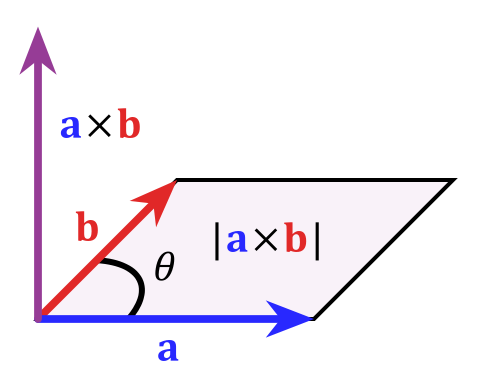
\includegraphics[scale=0.4,keepaspectratio=true]{./Bilder/480px-Cross_product_parallelogram.png}
 % 480px-Cross_product_parallelogram.png: 0x0 pixel, 0dpi, 0.00x0.00 cm, bb=
 \caption{Das Kreuzprodukt zweier Vektoren}
 \label{fig:Kreuzprd}
\end{wrapfigure}

Das Kreuzprodukt ist eine Verknüpfung, die im zwei Vektoren wieder einen Vektor zuordnet. Um es von anderen Produkten, insbesondere vom Skalarprodukt, zu unterscheiden, wird es mit einem Malkreuz als Multiplikationszeichen geschrieben.
Das Kreuzprodukt der Vektoren $\vec a$ und $\vec b$ ist ein Vektor, der senkrecht auf der von den beiden Vektoren aufgespannten Ebene steht und mit ihnen ein Rechtssystem bildet. Die Länge dieses Vektors entspricht dem Flächeninhalt des Parallelogramms, das von den Vektoren $\vec a$ und $\vec b$ aufgespannt wird.
\begin{mydef}
 Das Krauzprodukt ist definiert als:
    \[\vec{a}\times\vec{b} = \begin{pmatrix}a_1 \\ a_2 \\ a_3\end{pmatrix} \times \begin{pmatrix}b_1 \\ b_2 \\ b_3 \end{pmatrix} = \begin{pmatrix} a_2b_3 - a_3b_2 \\ a_3b_1 - a_1b_3 \\ a_1b_2 - a_2b_1 \end{pmatrix} \]
\end{mydef}

\subsection{Projektion}
Trifft Licht auf einen Körper, so wird es absorbiert oder reflektiert. Dadurch entsteht in der Grundebene ein Schatten des Körpers. Genau dies ist das Prinzip der Projektion.
\subsubsection{Parallelprojektion}
\begin{figure}[h!]
 \centering
 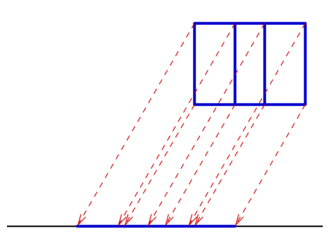
\includegraphics[scale=0.5,keepaspectratio=true]{./Bilder/parallelproj.jpg}
 % parallelproj.jpg: 0x0 pixel, 0dpi, nanxnan cm, bb=
 \caption{Die Parallelprojektion}
 \label{fig:parallelproj}
\end{figure}

\begin{mydef}
Eine Parallelprojektion ist eine Abbildung von Punkten des dreidimensionalen Raums auf Punkte einer gegebenen Ebene, wobei die Projektionsstrahlen zueinander parallel sind.
\end{mydef}
Vergleich: Sonnenstrahlen aus größter Entfernung.\\
Sei $\vec{v} = \begin{pmatrix} a \\ b \\ c \end{pmatrix}$ der Richtungsvektor der Parallelprojektion. Ein Bildpunkt $P$ hat den Ortsvektor $\begin{pmatrix} x_1 \\ x_2 \\ x_3 \end{pmatrix}$. Die Gerade der Projektion lautet dann $\vec{x} = \begin{pmatrix} x_1 \\ x_2 \\ x_3 \end{pmatrix} + r \cdot \begin{pmatrix} a \\ b \\ c \end{pmatrix}$. Der Bildpunkt $P'$ ergibt sich durch Bestimmung des Schnittpunktes der Geraden mit der Projektionssebene. Ist dies beispielsweise die $xy$-Ebene, so muss der Schnittpunkt $P'$ bei $(p \mid q\mid 0)$ sein. Man berechnet das $r$ für $x_3 = 0$ und löst damit die anderen Koordinaten.

\subsubsection{Zentralprojektion}
\begin{figure}[h!]
 \centering
 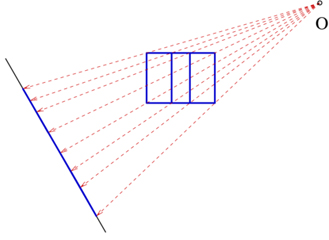
\includegraphics[scale=0.5,keepaspectratio=true]{./Bilder/zentrproj.jpg}
 % parallelproj.jpg: 0x0 pixel, 0dpi, nanxnan cm, bb=
 \caption{Die Zentralprojektion}
 \label{fig:zentrproj}
\end{figure}
\begin{mydef}
Im Gegensatz zur Parallelprojektion, wo man parallele Strahlen zur Projektion auf eine Ebene (Bildtafel) verwendet, benutzt man bei der Zentralprojektion Geraden durch einen festen Punkt $O$, dem Fluchtpunkt. 
\end{mydef}
Vergleich: Scheinwerferlicht.\\
Die Methode entspricht die der Parallelprojektion, nur die Gerade der Projektion wird definiert als Gerade zwischen $O$ und $P$.
 
%--------------------------------------------------------------------------------------------
%--------------------------------------------------------------------------------------------
%--------------------------------------------------------------------------------------------
%--------------------------------------------------------------------------------------------
%--------------------------------------------------------------------------------------------
%--------------------------------------------------------------------------------------------
%--------------------------------------------------------------------------------------------
%--------------------------------------------------------------------------------------------
%--------------------------------------------------------------------------------------------
%--------------------------------------------------------------------------------------------
%--------------------------------------------------------------------------------------------
%--------------------------------------------------------------------------------------------
\clearpage

\part{Informatik}
\chapter{Software-Engineering}\index{Softwaretechnik}\index{Software-Engineering}
\dictum[Linus Torvalds]{Wenn du dir die Anwender deiner Programme als Idioten vorstellst, werden auch nur Idioten deine Programme verwenden.}

Softwaretechnik beschäftigt sich mit der Herstellung bzw. Entwicklung von Software, der Organisation und Modellierung der zugehörigen Datenstrukturen und dem Betrieb von Softwaresystemen.
Balzert beschreibt die Softwaretechnik als ``Zielorientierte Bereitstellung und systematische Verwendung von Prinzipien, Methoden und Werkzeugen für die arbeitsteilige, ingenieurmäßige Entwicklung und Anwendung von umfangreichen Softwaresystemen''\cite{Balzert1996}. \\
Doch was muss ein gutes System ausmachen?
Letztendlich ist ein gutes System eines, das den Bedürfnissen des Anwenders gerecht wird.
Das System muss deshalb... \cite{Andelfinger2005}
\begin{description}
\item[nützlich und nutzbar]  sein. Es muss dem Anwender das Leben möglichst stark erleichtern.
\item[zuverlässig] sein. Es soll möglichst wenig Fehler enthalten.
\item[flexibel] sein. Das System muss leicht an geänderte Anforderungen des Benutzers anpassbar sein. Die Fehler müssen leicht zu beheben sein.
\item[kostengünstig]  sein, nicht nur in der Anschaffung, sondern auch im Unterhalt.
\item[verfügbar] sein. Das System muss auf jetzigen und zukünftigen Zielplattformen (Hardware, Betriebssystemen etc.) lauffähig bzw. leicht adaptierbar sein. Zur Verfügbarkeit gehört natürlich auch, dass das Softwareprodukt überhaupt existiert und zwar zu dem Zeitpunkt, zu dem es zum Einsatz kommen soll.
\end{description}
\newpage
\section{Phasen der Softwareentwicklung}
In der Softwaretechnik läuft der Entwicklungsprozess eines Softwareprojektes in Phasen ab. Es gibt verschiedene Phasenmodelle, die auch die Zusammenarbeit zwischen den verschienden Beiteiligten regeln. \\
Das Urmodell ist das so genannte Wasserfallmodell\index{Wasserfallmodell}, welches ein rein sequenzielles Vorgehen vorsah:
\begin{figure}[h!]
 \centering
 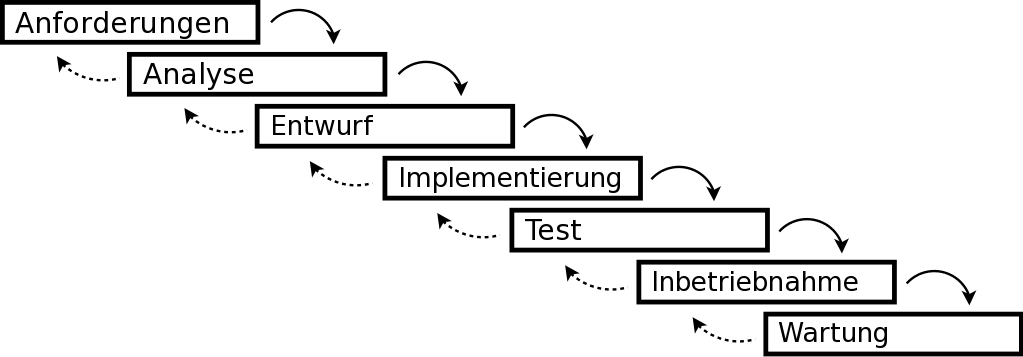
\includegraphics[scale=0.8,keepaspectratio=true]{./Bilder/wmodell.png}
 % wmodell.png: 0x0 pixel, 0dpi, nanxnan cm, bb=
 \caption{Das Wasserfallmodell}
 \label{fig:Wasserfallmodell}
\end{figure}

Das Spiralmodell\index{Spiralmodell} hingegen, ist ein generisches Vorgehensmodell, bei dem das Management immer wieder eingreifen kann, da man sich spiralförmig voran entwickelt:
\begin{figure}[h]
 \centering
 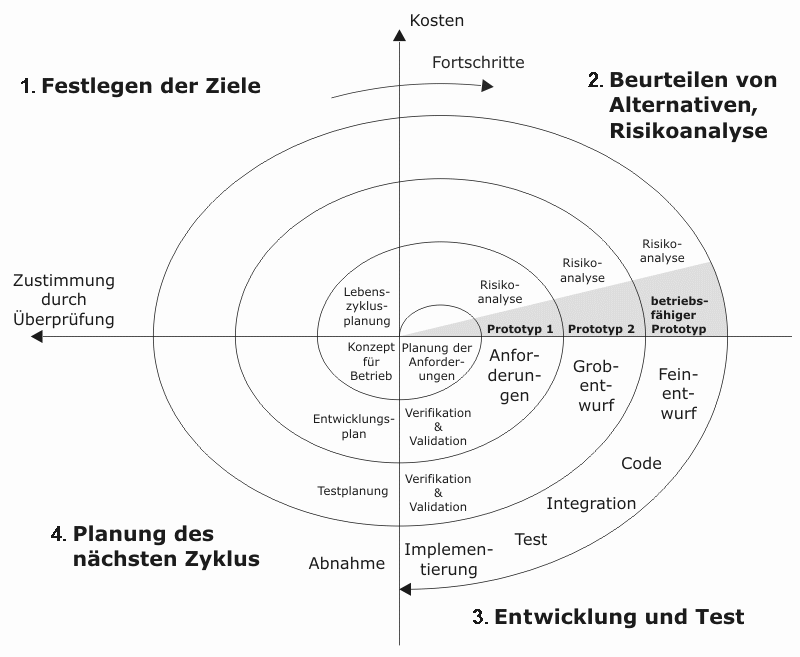
\includegraphics[scale=0.4,keepaspectratio=true]{./Bilder/Spiralmodel_nach_Boehm.png}
 % Spiralmodel_nach_Boehm.png: 0x0 pixel, 0dpi, nanxnan cm, bb=
 \caption{Spiralmodell nach Boehm}
 \label{fig:Spiralmodell}
\end{figure}


\section{UML}

\lstset{
  basicstyle=\footnotesize,
  frame=single,
  identifierstyle=\color{black},
  keepspaces=true,
  keywordstyle=\color{red},
  language=java,
  numbers=left,
  numberstyle=\tiny\color{gray},
  stringstyle=\color{blue}
}

Die \textbf{Unified Modeling Language} (Vereinheitlichte Modellierungssprache), kurz UML, ist eine grafische Modellierungssprache zur Spezifikation, Konstruktion und Dokumentation von Software-Teilen und anderen Systemen. Bei Modellierung handelt es sich um eine partielle, subjektive Abbildung eines Abschnitts der realen Welt. \cite{Kluth2011}
In der UML gibt es folgende Diagramme:
\begin{itemize}
\item Strukturdiagramme
\begin{itemize}
  \item Klassendiagramm -Class Diagram
  \item Objektdiagramm - Object Diagram
  \item Komponentendiagramm - Component Diagram
  \item Paketdiagramm - Package Diagram
  \item Kompositionsstrukturdiagramm - Composite Structure Diagram
  \item Verteilungsdiagramm - Deployment Diagram
\end{itemize}
  \item Verhaltensdiagramme
\begin{itemize}
  \item Aktivitätsdiagramm - Activity Diagram
  \item Anwendungsfalldiagramm - Use Case Diagram 
  \item Zustandsdiagramm -State Machine Diagram
  \item Interaktionsdiagramme
  \begin{itemize}
  \item Interaktionsübersichsdiagramm - Interaction Overview Diagram
  \item Sequenzdiagramm - Sequence Diagram
  \item Kommunikationsdiagramm - Communication Diagram
  \item Zeitverlaufsdiagramm - Timing Diagram
  \end{itemize}
\end{itemize}
\end{itemize}

\subsection{Das Klassendiagramm}
Klassendiagramme stellen die statische Struktur eines Systems dar. Sie zeigen die Klassen, die Eigenschaften der Klassen (Attribute), das Verhalten (Operationen)  der Klassen und die Beziehungen zwischen den Klassen. Sie sind der zentrale Diagrammtyp der UML und werden in allen Phasen der Softwareentwicklung eingesetzt. Die Notation lautet wie folgt:
\begin{figure}[h]
 \centering
 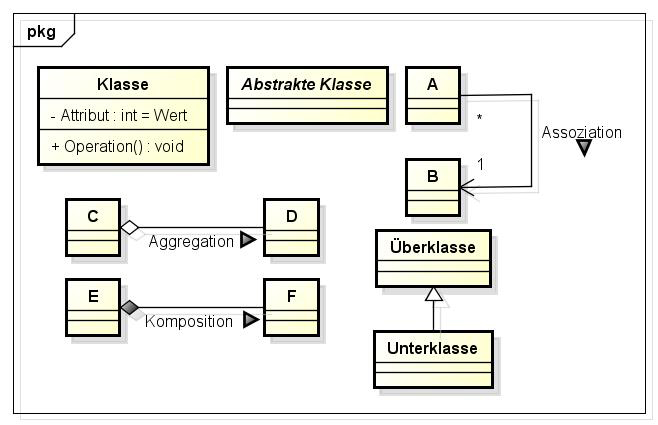
\includegraphics[scale=0.55,keepaspectratio=true]{./Bilder/classdiagr.jpg}
 % classdiagr.jpg: 0x0 pixel, 0dpi, nanxnan cm, bb=
 \caption{Beispiel-Klassendiagramm}
 \label{fig:Klassendiagramm}
\end{figure}

\subsubsection{Die Klasse}
Eine Klasse kann als Rechteck dargestellt werden, das den Klassennamen enthält. Üblicherweise bestehen Klassen aus drei Bereichen; der obere Bereich enthält den Stereotyp, das Paket zu dem die Klasse gehört und den Namen. Im mittleren Bereich werden die Attribute angegeben und im unteren Bereich stehen die Operationen der Klasse.
Die Syntax für die Deklaration von Attributen lautet: \[[Sichtbarkeit] Name [:Typ] [=Wert]\]
Die Syntax für die Deklaration von Operationen lautet :  \[[Sichtbarkeit] Name [(Parameterliste)] [: Returntyp]\] 
Dabei gibt die Sichtbarkeit an, wie die Sichtbarkeit eines Elementes relativ zu seiner Umgebung ist. Die Sichtbarkeit gibt also an,  welche Elemente auf ein Attribut, bzw. auf eine Operation zugreifen können. Der Zugriff auf ein Attribut definiert den lesenden und schreibenden Zugriff auf das Attribut; die Sichtbarkeit von Operationen gibt an,   welche   Elemente   die   Operation   aufrufen   können.   Folgende Sichtbarkeitsmodi sind definiert:
\begin{description}
 \item[public] Jedes andere Element hat Zugriff.
 \item[private] Der Zugriff ist auf die Objekte der Klasse selbst beschränkt
 \item[protected] Zugriff besteht nur für die definierende Klasse und die Vererbungslinien, die von ihr ausgehen.
 \item[package] Das Element ist sichtbar für alle Klassen, die sich im selben Paket befinden.
\end{description}
\begin{lstlisting}[caption=Implementierung Klasse]
public class Klasse
{
  private int Attribut;
  public void Operation() {
  [...]
}
\end{lstlisting}

\subsubsection{Abstrakte Klasse}
Der Name einer abstrakten Klasse wird kursiv geschrieben. Alternativ kann die Eigenschaft {abstract} angegeben werden.
\begin{lstlisting}[caption=Implementierung abstrakte Klasse]
public abstract class AbstrakteKlasse [...]
\end{lstlisting}
Es gibt zudem auch noch statische Klassen \& Attribute, welche in der UML unterstrichen dargestellt werden.


\subsubsection{Die Assoziation}
Eine Linie zwischen den Klassen stellt eine Assoziation dar. Eine Assoziation ist eine Beziehung zwischen Klassen. Die Objekte der Klassen kommunizieren über die Assoziationen miteinander. Die Assoziation kann einen Namen haben. Ein Pfeil an dem  Assoziationsnamen  gibt die Leserichtung  des Namens an. An den Assoziationsenden können die Rollen der beteiligten Klassen und die Multiplizität angegeben werden. 
Mit einem Pfeil an der Assoziation kann die Navigationsrichtung angegeben werden. Der Pfeil drückt die Zugriffsrichtung der Objekte aus. Objekt A greift auf B zu, B greift nie auf A zu. Die Impelemtationsmöglichkeiten hängen von der Situation und Multiplizität ab. 


\subsubsection{Vererbung}
Die Vererbung ist ein Grundkonzept objektorientierter Programmiersprachen und dient der Wiederverwendung von Quellcode. Sie wird verwendet um Eigenschaften einer Oberklasse an Unterklassen zu vererben. Alle Eigenschaften (Attribute und Operationen) der Oberklasse, die für die Unterklasse sichtbar sind, werden an diese vererbt. Sie sind in der Unterklasse benutzbar, als wären sie in der Klasse selbst definiert. Die Unterklassen dürfen weitere, speziellere Eigenschaften haben. Aus der Sichtweise der Oberklasse sind die Unterklassen immer speziellere Klassen; aus der Sichtweise der Unterklassen ist die Oberklasse die allgemeinere, generellere Klasse. Deshalb wird die Vererbung auch Generalisierung oder Spezialisierung genannt. Vererbungsbeziehungen werden mit einem Pfeil dargestellt. Die  Pfeilspitze zeigt auf die Oberklasse. Die Oberklasse vererbt ihre Eigenschaften an die Unterklasse(n).
\begin{lstlisting}[caption=Implementierung Vererbung]
public class Oberklasse { [...] }
public class Unterklasse extends Oberklasse { [...] }
\end{lstlisting}

\subsubsection{Aggregation}
Die Aggregation wird verwendet um zwischen Klassen eine Teile-Ganzes-Beziehung aufzubauen. Die Raute befindet sich an dem Ende des Ganzen. Die Aggregation ist eine spezielle Art der Assoziation. Da das Ganze die Teile enthält, sollten am  Assoziationsende der Teile ein Navigationspfeil stehen. Da die Aggregation eine Spezialform der Assoziation ist, wird sie wie eine Assoziation implementiert. - Je nach Multiplizitäten.

\subsubsection{Komposition}
Die Komposition als Sonderfall der Aggregation beschreibt ebenfalls die Beziehung zwischen einem Ganzen und seinen Teilen. Der Unterschied zur Aggregation ist, dass die Existenz eines Objekts, das Teil eines Ganzen ist, von der Existenz des Ganzen abhängig ist. Ein Objekt kann dabei immer nur Teil maximal eines Ganzen sein (Multiplizität 0..1 oder 1). \\
In Java gibt es verschiedene Möglichkeiten, eine Komposition zu implementieren. Dabei ist jedoch keine Optimal, da sich die Funtkionsweise von Java mit der erwünschten Umsetzung der Komposition widerspricht.
\begin{enumerate}
 \item $a$ erschafft $b$, damit kein Anderer $b$ kennt; $a$ verwendet den Konstruktor von $b$ mit ``einfachen'' Datentypen
 \item Wir legen eine Kopie des enthaltenen Objektes an
 \item Klasse $B$ wird in $A$ definiert
\end{enumerate}
Die Beispielhafte Implementation erfolgt folgendermaßen:
\begin{enumerate}
 \item :
  \begin{lstlisting}[caption=Implementierung durch Erschaffung des Teils vom Ganzen]
    public class Ganzes
    {
      Teil b1, b2;
      public Ganzes(...)
       {
	  b1 = new Teil(...);
	  b2 = new Teil(...);
       }
    }
    public class Teil{ [...] }
  \end{lstlisting}
 \item :
  \begin{lstlisting}[caption=Implementierung durch Anlegen einer Kopie]
    public class Ganzes
    {
      Teil b1, b2;
      public Ganzes(Teil b1, Teil b2)
       {
	  this.b1 = new Teil(b1);
	  this.b2 = new Teil(b2);
       }
    }
    public class Teil
    {
      public Teil(Teil t)
      {
	//kopiere das übergebene Objekt t
      }
    }
  \end{lstlisting}
 \item :
  \begin{lstlisting}[caption=Implementierung durch enthaltene Klassen]
    public class Ganzes
    {
      public class Teil{ [...] }
      Teil b1, [...]
    }
  \end{lstlisting}
\end{enumerate}





\chapter{Sortieralgorithmen}
Teilweise übernommen aus www.sortieralgorithmen.de.
\section{Bubblesort}
Der Name "Bubblesort" kommt von bubble (dt. Blase), da man seine Funktionsweise sehr gut anhand von langsam aufsteigenden Luftblasen in einer Wassersäule erklären kann.
\begin{lstlisting}[caption=Bubblesort]
public static int[] bubblesort(int[] zusortieren) {
  int temp;
  for(int i=1; i<zusortieren.length; i++) {
    for(int j=0; j<zusortieren.length-i; j++) {
      if(zusortieren[j]>zusortieren[j+1]) {
	temp=zusortieren[j];
	zusortieren[j]=zusortieren[j+1];
	zusortieren[j+1]=temp;
      }
    }
  }
  return zusortieren;
}
\end{lstlisting}
Ein Feld wird einmal vollständig durchlaufen. Dabei werden die jeweiligen Nachbarelemente miteinander verglichen und ggf. ausgetauscht. Am Ende befindet sich das größte Element am Ende des Feldes. Dieser Schritt wird nun mit dem kleineren Teilfeld (Feld ohne das letzte Element) wiederholt und wiederholt und ... Und irgendwann sind wir fertig und die Elemente sind sortiert.\\
In einer Wassersäule befinden sich unterschiedlich große Luftblasen. Die unterste Luftblase steigt nun langsam auf. Während sie an kleineren problemlos vorbeikommt, wird sie durch größere gestoppt. Durch den Zusammenprall setzt sich die größere Luftblase in Bewegung, bis auch diese gestoppt wird oder am oberen Säulenende ankommt. Nun setzt sich abermals die unterste Luftblase in Bewegung bis ... Und wenn die Wassersäule eine endliche Anzahl Luftblasen enthält, dann kann irgendwann keine Luftblase mehr aufsteigen, da sich über ihr eine noch größere befindet. Die Luftblasen sind dann der größe nach von unten (klein) nach oben (groß) sortiert.\\
Eine Seifenblase kann genau zwei Elemente in sich einschließen. Diese Seifenblase steigt nun langsam auf. Das schwerere der beiden Elemente in der Blase kann nicht nach oben getragen werden und fällt unten raus, während oben ein neues Element hineinkommt. Dadurch trägt die Seifenblase das leichteste Element bis ganz nach oben. Hier zerplatzt die Seifenblase und unten entsteht eine neue.\\
Aufgrund der Vergleiche benachbarter Elemente wird dieses Verfahren auch als ``Sortierung durch Nachbarvergleiche'' bezeichnet.

\section{Selectionsort}
Der Name "Selectsort" kommt von selection (dt. Auswahl), da in jedem Schritt das größte (oder kleinste) Element selektiert wird.
\begin{lstlisting}[caption=Bubblesort]
public static int[] selectionsort(int[] zusortieren) {
  for (int i = 0; i < zusortieren.length - 1; i++) {
    for (int j = i + 1; j < zusortieren.length; j++) {
      if (zusortieren[i] > zusortieren[j]) {
	int temp = zusortieren[i];
	zusortieren[i] = zusortieren[j];
	zusortieren[j] = temp;
      }
    }
  }
  return zusortieren;
}
\end{lstlisting}
Ein Feld wird einmal vollständig durchlaufen. Dabei wird durch einfache Vergleiche das größte Element herausgesucht (selektiert) und zum Schluss an das Feldende gepackt. Dieser Schritt wird nun mit dem kleineren Teilfeld (Feld ohne das letzte Element) wiederholt und wiederholt und ... Und irgendwann sind wir fertig und die Elemente sind sortiert.\\
Aufgrund der Auswahl von Elementen wird dieses Verfahren auch als ``Sortierung durch Auswahl'' bezeichnet.

\section{Insertionsort}
Der Name "Insertsort" kommt von insertion (dt. Einfügen), da in jedem Schritt ein Element in eine bereits sortierte Gruppe von Elementen eingefügt wird.
\begin{lstlisting}[caption=Bubblesort]
public static int[] insertionSort(int[] zusortieren) {
  int temp;
  for (int i = 1; i < zusortieren.length; i++) {
    temp = zusortieren[i];
    int j = i;
      while (j > 0 && zusortieren[j - 1] > temp) {
	zusortieren[j] = zusortieren[j - 1];
	j--;
      }
    zusortieren[j] = temp;
  }
  return zusortieren;
}
\end{lstlisting}
Ein kleineres bereits sortiertes Teilfeld wird um ein Element erweitert. Dieses neu hinzugekommene Element wird durch Vergleiche und Verschiebungs- oder Vertauschungsoperationen an die ``richtige'' Stelle dieses größeren Teilfeldes eingefügt. Dieser Schritt wird wiederholt, bis das Teilfeld maximal ist (also dem Gesamtfeld entspricht). Dann sind wir fertig und die Elemente sind sortiert.\\
Bei einem Kartenspiel bekommt man nacheinander eine bestimmte Anzahl von Karten ausgehändigt. Erst hat man eine in der Hand, dann werden es zwei, drei, vier, ... Damit man da den Überblick behält sorgt man am besten dafür, daß die Karten sortiert in der Hand liegen. Kommt eine neue Karte hinzu, wird diese direkt an die richtige Position gesteckt.\\
Aufgrund des Einfügens von Elementen in eine sortierte Menge wird dieses Verfahren auch als ``Sortierung durch Einfügen'' bezeichnet.

\section{Quicksort}
Der Name "Quicksort" kommt von quick (dt. schnell) und spielt auf sein (in der Regel) phantastisches Laufzeitverhalten an.
\begin{lstlisting}[caption=Quicksort mit Privot-Element rechts]
public void quickSort(int links, int rechts, int feld[]) { 
  int i=links, j=rechts-1; 
  int pivot; 
  if (rechts>links) { 
    pivot = feld[rechts]; 
    while (i<j) { 
      while (feld[i] < pivot && i < rechts) {i++;} 
      while (feld[j] > pivot && j > links)  {j--;} 
      if(i<j) exchange(i,j,feld); 
    } 
  exchange(i,rechts,feld); 
  quickSort(links,i-1, feld); 
  quickSort(i+1,rechts, feld); 
  } 
} 
\end{lstlisting}
Ein Feld wird in zwei (in der Regel unterschiedlich große) Teilfelder aufgeteilt, die Elemente werden dabei so vertauscht, daß alle Elemente des linken Teilfeldes kleiner (oder gleich) den Elementen des rechten Teilfeldes sind. Die einzelnen Teilfelder werden dann wieder sortiert... Und irgendwann sind wir fertig und das gesamte Feld liegt sortiert vor.\\
Die Aufteilung eines Feldes in zwei Teilfelder geschieht aufgrund von Vergleichen mit einem speziellen (Am Anfang der Teilung gewählten) Pivotelement. Deshalb wird dieses Verfahren auch als ``Sortierung durch Pivotisierung'' oder ``Sortierung durch Partitionierung'' bezeichnet.




\section{Laufzeitanalyse}
\subsection{Die O-Notation}
Für die Effizienzanalyse von Algorithmen wird eine spezielle mathematische Notation verwendet, die als O-Notation bezeichnet wird. Die O-Notation erlaubt es, Algorithmen auf einer höheren Abstraktionsebene miteinander zu vergleichen. Algorithmen können mit Hilfe der O-Notation unabhängig von Implementierungsdetails, wie Programmiersprache, Compiler und Hardware-Eigenschaften, verglichen werden.
\begin{mydef}
 Die Funktion $T(n) = O(g(n))$, wenn es positive Konstanten $c$ und $n_{0}$ gibt, so dass $T(n) \leq c \cdot g(n)$ für alle $n \geq n_{0}$.
\end{mydef}
Wichtig ist, dass  $O(n^2)$  eine Menge darstellt, weshalb die Schreibweise $2n + n^2 \in O(n^2)$ besser ist als die Schreibweise $n^2 + 2n = O(n^2)$.
\subsubsection{Klassifikation von Algorithmen}
\begin{center}
\begin{tabularx}{\columnwidth}{|l|l|X|} \hline 
\textbf{Notation} & \textbf{Komplexitätsklasse} & \textbf{Anschauliche Beschreibung}\\ \hline \hline 
$O(1)$ & konstant & Die meisten Anweisungen in einem Programm werden nur 
einmal oder eine konstante Anzahl von Malen wiederholt. \\ \hline 
$O(log n)$ & logarithmisch & Verdoppelt sich das Argument\footnote{Beispielsweise die Länge eines zu sortierenden Arrays}, wächst die Laufzeit um ca. einen konstanten Betrag.\\ \hline 
$O(n)$ & linear & Verdoppelt sich das Argument, verdoppelt sich auch die ungefähre Laufzeit.\\ \hline 
$O(n^2)$ & quadratisch & Verdoppelt sich das Argument, vervierfacht sich die ungefähre Laufzeit.\\ \hline 
$O(2^n)$ & exponentiell & Erhöht sich das Argument um eins, verdoppelt sich die ungefähre Laufzeit. \\ \hline 
\end{tabularx}
\end{center}

\subsection{Stabilität von Sortieralgorithmen}
\begin{mydef}
 Ein stabiles Sortierverfahren ist ein Sortieralgorithmus, der die \textit{Reihenfolge der Datensätze, deren Sortierschlüssel gleich sind, bewahrt}.
\end{mydef}
Wenn bspw. eine Liste alphabetisch sortierter Personendateien nach dem Geburtsdatum neu sortiert wird, dann bleiben unter einem stabilen Sortierverfahren alle Personen mit gleichem Geburtsdatum alphabetisch sortiert.

\subsection{Zusammenstellung der beschriebenen Sortieralgorithmen}
\begin{center}
\begin{tabular}{l|cc|c}
Algorithmus   & \multicolumn{2}{c|}{Laufzeitklasse} & stabil? \\ 
              & worst     & best     &  \\ \hline
BubbleSort    & $n^2$     & $n$      &  $\checkmark$ \\
SelectionSort & $n^2$     & $n^2$    &  $\checkmark$ \\
InsertSort    & $n^2$     & $n$      &  $\checkmark$ \\
QuickSort     & $n log n$ & $n log n$ & $\diagup$      
\end{tabular}
\end{center}

\chapter{Dynamische Datenstrukturen}
tbd

\chapter[Modellation und Implementation von Netzwerkanwendungen]{Modellieren  und Implementieren  kontextbezogener  Problemstellungen als 
Netzwerkanwendungen}
\section{Netzwerkprotokolle}
tbd
\subsection{TCP/IP-Referenzmodell}
tbd
\section{Kryptologie}
Die Kryptologie ist die Wissenschaft der Verschlüsselung und der Entschlüsselung von Informationen. Auch die Analyse der unterschiedlichen kryptografischen Verfahren, d. h ihre Stärken und Schwächen, zählt zur Kryptologie. \\
In der Kryptologie gibt es wie in der Netzwerktechnik ein Schichtenmodell, mit Ebenen, die auf einander Aufbauen und voneinander abhängig sind:\\
\begin{center}
\begin{tabular}{c}
Bedrohungen\\
Ziele\\
Protokolle\\
Mechanismen\\
kryptogr. Algorithmen
\end{tabular}
\end{center}

\subsection{Schutzziele}
In der Informatik gibt es bestimmte Dinge, die man vor Angriffen schützen will. Die klassischen Schutzziele sind:\footnote{Entnommen aus \cite{Kluth2011}} \\

\paragraph{Verfügbarkeit} eines Dienstes, den man anbietet sollte auch tatsächlich gewährleistet sein. Denial of Service Attacken versuchen gerade dies zu verhindern. Ein konkretes Beispiel mit dem damit verbundenen wirtschaftlichen Schaden wäre, dass Sie
ein Produkt auf einer Auktionsplattform, sagen wir einen Sportwagen anbieten. Erfahrungsgemäß steigt der Preis vor allem in der letzten Stunde vor dem Ende der Auktion. Wie würden Sie reagieren, wenn die Auktionsplattform in der letzten Stunde nicht verfügbar ist und ihr Wagen für den Spottpreis von 100 Euro den
Besitzer wechselt? Wie stände es mit dem allgemeinen Vertrauen in eine solche Auktionsplattform?

\paragraph{Vertraulichkeit} bedeutet, dass bestimmte Informationen nur berechtigten Personen auch Verfügung stehen. Dies betrifft natürlich auch Nachrichten die über öffentliche Netze versandt werden.

\paragraph{Integrität} bedeutet, dass Informationen nicht von Unbefugten unberechtigt und unbemerkt verändert werden. Ob diese Informationen veprtraulich sind oder nicht, spielt hierbei keine Rolle. Beim Betreiben einer Webseite haben Sie in der Regel ein großes Interesse an Öffentlichkeit. Sie wären aber sicherlich nicht erfreut für ungewollt für ein zwielichtiges Produkt zu werben.

\paragraph{Verbindlichkeit} ist eigentlich kein klassisches Schutzziel, sondern ist erst im letzten Jahrzehnt bedingt durch digitale Signaturen hinzugekommen. Es bedeutet, dass der Sender einer Information später nicht leugnen kann, dass diese Information von ihm versendet wurde. Dies ist z.B. beim Kauf von Produkten im Netz für den Verkäufer ein interessantes Thema.
 
\subsection{Protokolle} 
Ein Protokoll ist ein verteilter Algorithmus, der durch eine Folge von Schritten definiert wird, die exakt die Aktionen spezifiziert, die zwei oder mehr Partner ausführen müssen, um ein bestimmtes Sicherheitsziel zu erreichen. Chiffren, digitale Signaturen, Einweg-Hashfunktionen, Pseudozufallszahlen-Generatoren sind wichtige Werkzeuge bzw. Bausteine, die genutzt werden können, um Protokolle aufzubauen. \\
Die Verwendung sicherer kryptographischer Bausteine garantiert keineswegs ein sicheres Protokoll. Ein \textbf{Protokoll- oder Mechanismus-Fehler} liegt vor, wenn es einem Angreifer gelingt, ein mit dem Protokoll bzw. Mechanismus angestrebtes Sicherheitsziel zu vereiteln, ohne daß er dazu die als Basis verwendeten Algorithmen (z.B. Chiffren und Einweg-Hashfunktionen) brechen muss. Real eingesetzte Protokolle sind deshalb sehr sorgfältig zu entwerfen und zu implementieren, wobei es auf die kleinsten Details ankommen kann. 
Zur Vermeidung unnötiger Risiken sollte man Protokolle und deren Implementierungen (Programme und Bibliotheken) einsetzen, die einer gründlichen öffentlichen Analyse unterzogen wurden und die allgemein als sicher angesehen werden. \\
\texttt{TBD: Beispiel für Protokolle}

\subsection{Mechanismen}
Kryptologische Mechanismen bezeichnen die Art der kryptografischen Algorithmen, die in den Protokollen verwendet werden.\\ Die wichtigsten sind:

\subsubsection{Symmetrische Verschlüsselung}
Beide Teilnehmer verwenden bei einer symmetrischen Verschlüsselung den selben Schlüssel, sowohl um den Klartext zu verschlüsseln, als auch um den Ciphertext wieder zu entschlüsseln. Bei einigen Verfahren sind die Schlüssel zwar nciht die Selben, können jedoch auf einfachste Art aus dem jeweiligen Gegenschlüssel berechnet werden.
\begin{wrapfigure}{r}{0.5\textwidth}
 \centering
 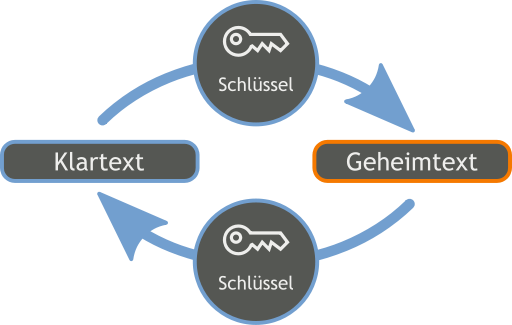
\includegraphics[bb=0 0 512 325,scale=0.35,keepaspectratio=true]{./Bilder/512px-Orange_blue_symmetric_cryptography_de.png}
 \caption{Verschlüsselung und Entschlüsselung mit dem gleichen Schlüssel}
 \label{fig:SymmV}
\end{wrapfigure}
Der große Nachteil symmetrischer Verfahren liegt in der Nutzung ein- und desselben Schlüssels zur Ver- und Entschlüsselung, d. h. neben der verschlüsselten Information muss auch der Schlüssel übermittelt werden. Das Problem beim Einsatz symmetrischer Verfahren ist, dass der Schlüssel über einen sicheren Kanal übertragen werden muss, denn die Sicherheit des Verfahrens hängt von der Geheimhaltung des Schlüssels ab. Früher wurde der Schlüssel typischerweise durch einen Boten persönlich überbracht. Seit den 1970er Jahren sind mit dem Diffie-Hellman-Schlüsselaustausch asymmetrische Schlüsselaustauschprotokolle bekannt, mit denen auch über einen abgehörten Kanal Schlüssel sicher übertragen werden können. Eine weitere Möglichkeit ist der Einsatz asymmetrischer Verschlüsselungsverfahren um den symmetrischen Schlüssel selbst zu verschlüsseln und ihn so geschützt auch über einen unsicheren Kanal übertragen zu können. Bei der Kommunikation können mit dieser hybriden Verschlüsselung also die Vorteile (beispielsweise die höhere Geschwindigkeit) der symmetrischen Verschlüsselung ausgenutzt werden, während der Schlüssel durch die asymmetrische Verschlüsselung vor dem Zugriff eines Angreifers geschützt wird.

\subsubsection{Asymmetrische Verschlüsselung}
Beide Teilnehmer verwenden bei einem asymmetrischen Verschlüsselungsverfahren im Gegensatz zu symmetrischen Verschlüsselungen keinen gemeinsamen geheimen Schlüssel. Ein Benutzer erzeugt ein Schlüsselpaar, das aus einem privaten Schlüssel und einem öffentlichen Schlüssel besteht. Der öffentliche Schlüssel ermöglicht es jedem, Daten für den Inhaber des privaten Schlüssels zu verschlüsseln, oder ihn zu authentifizieren. Der private Schlüssel ermöglicht es seinem Inhaver, mit dem öffentlchen Schlüssel verschlüsselte Daten zu entschlüsseln oder digitale Signaturen zu erzeugen.
\begin{figure}[h!]
 \centering
 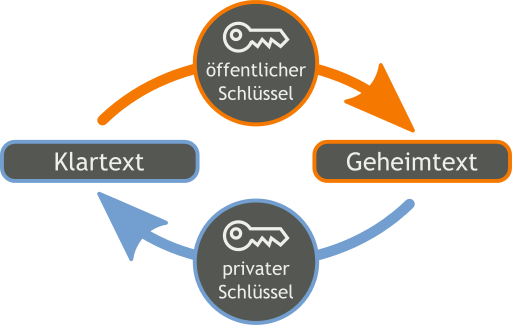
\includegraphics[bb=0 0 512 325,scale=0.4,keepaspectratio=true]{./Bilder/Orange_blue_public_key_cryptography_de.png}
 % Orange_blue_public_key_cryptography_de.png: 512x325 pixel, 72dpi, 18.06x11.47 cm, bb=0 0 512 325
 \caption{Verschlüsselung mit öffentlichem Schlüssel und Entschlüsselung mit privatem Schlüssel}
 \label{fig:asyV}
\end{figure}
Der entscheidende Vorteil von asymmetrischen Verfahren ist, dass sie das Schlüsselverteilungsproblem vermindern. Bei symmetrischen Verfahren muss vor der Verwendung ein Schlüssel über einen sicheren, d. h. abhörsicheren und manipulationsgeschützten, Kanal ausgetauscht werden. Da der öffentliche Schlüssel nicht geheim ist, muss bei asymmetrischen Verfahren der Kanal nicht abhörsicher sein; wichtig ist nur, dass der öffentliche Schlüssel dem Inhaber des dazugehörigen geheimen Schlüssels zweifelsfrei zugeordnet werden kann. Dazu kann beispielsweise eine vertrauenswürdige Zertifizierungsstelle ein digitales Zertifikat ausstellen, welches den öffentlichen Schlüssel dem privaten Schlüssel(inhaber) zuordnet. Als Alternative dazu kann auch ohne zentrale Stelle durch gegenseitiges Zertifizieren von Schlüsseln ein sog. Web of Trust aufgebaut werden.

\subsubsection{Hashfunktionen}
Eine \textbf{Hashfunktion} ist eine Abbildung, die eine große Eingabemenge (die Schlüssel) auf eine kleinere Zielmenge (die Hashwerte) abbildet – sie ist daher nicht injektiv. Dabei kann die Eingabemenge auch Elemente mit unterschiedlichen Längen enthalten, die Elemente der Zielmenge haben dagegen meist eine feste Länge. In der Kryptologie werden Hashfunktionen verwendet, um den Inhalt übertragener Daten zu verifizieren. Hier wird daher zusätzlich gefordert, dass Kollisionen sehr schwer zu finden sind, damit modifizierte Daten nicht zufällig den gleichen Hashwert besitzen wie das Original. Eine sog. „Kollision“ tritt dann auf, wenn zwei verschiedenen Eingabedaten derselbe Hashwert zugeordnet wird. Da die Menge der möglichen Hashwerte meist kleiner ist als die der möglichen Eingaben, sind solche Kollisionen dann prinzipiell unvermeidlich, weshalb es Verfahren zur Kollisionserkennung geben muss. Eine gute Hashfunktion zeichnet sich dadurch aus, dass sie für die Eingaben, für die sie entworfen wurde, möglichst wenige Kollisionen erzeugt.

\subsection{Kryptographische Algorithmen}
Wir definieren uns:
\begin{itemize}
 \item den Klartext $M$
 \item den Ciphertext $C$
 \item den Schlüssel $K$, beziehungsweise die Schlüsselpaare $(e,N)$ und $(d,N)$, wobei $e$ der öffentliche Schlüssel und $d$ der private Schlüssel ist.
 \item die Verschlüsselungsfunktion $C = E(M)$
 \item die Entschlüsselungsfunktion $M = D(C)$
\end{itemize}

\subsubsection{Caesar}
Die Caesar-Verschlüsselung ist ein symmetrisches, monoalphabetisches Verschlüsselungsverfahren. Bei der Verschlüsselung wird jeder Buchstabe des Klartexts auf einen Geheimtextbuchstaben abgebildet. Diese Abbildung ergibt sich, indem man die Zeichen eines geordneten Alphabets um eine bestimmte Anzahl zyklisch nach rechts verschiebt (rotiert). Die Anzahl der verschobenen Zeichen bildet den Schlüssel, der für die gesamte Verschlüsselung unverändert bleibt. \\
Man bildet alle Zeichen des gewünschten Alphabets auf einen Restklassenring ab. Dann gilt monographisch für jeden Buchstaben des Textes:
\[E_{K}(M) = (M+K) \mod{26}\]
\[D_{K}(C) = (C-K) \mod{26}\]
\subsubsection{Vigenère}
Die Vigenère-Verschlüsselung ist ein symmetrisches, polyalphabetisches Verschlüsselungsverfahren. Die Verschlüsselung arbeitet ähnlich wie die Caesar-Verschlüsselung. Der Schlüssel ist hier ein String von mehreren Buchstaben des verwendeten Alphabets. Jeder Buchstabe des Textes wird mit der Ordnung des jeweiligen Buchstabens des Schlüssels nach dem Caesar-Prinzip substituiert. \\
Verwendet man das Vigenère-Quadrat, kann man den Geheimtext direkt ablesen. Die Ordnung des Schlüssels und die des Textes stehen in der ersten Reihe und Spalte. Der Ciphertext befindet sich im Körper.\\
\begin{tikzpicture}
\foreach \i in {0,...,25} {
  \foreach \j in {0,...,25} {
    \edef\k{\ifnum\numexpr\i+\j\relax>25
        \the\numexpr\i+\j-26\relax
      \else
        \the\numexpr\i+\j\relax
      \fi}
  \node[draw,minimum size=0.5cm,inner sep=0pt]
    at (\i*0.5,-\j*0.5) {\strut\symbol{\numexpr`A+\k\relax}};
  }
  \node at (-0.5,-\i*0.5) {\strut\i};
  \node at (\i*0.5,0.5)   {\strut\i};
}
\end{tikzpicture}

\subsubsection{RSA}
Die RSA-Verschlüsselung ist ein asymmetrisches Verschlüsselungsverfahren. Es wird zunächst vom Empfänger der Nachricht ein Schlüsselpaar generiert.
\begin{enumerate}
 \item Wähle zufällig und stochastisch unabhängig zwei Primzahlen $p \neq q$.
 \item Berechne den RSA-Modul $N = p \cdot q$. 
 \item Berechne die Eulersche $\varphi$-Funktion von $N$: $\varphi(N) = (p-1) \cdot (q-1)$.
 \item Wähle eine zu $\varphi(N)$ teilerfremde Zahl $e$, für die gilt $1 < e < \varphi(N)$.
 \item Berechne den Entschlüsselungsexponenten $d$ als Multiplikatives Inverses von $e$ bezüglich des Moduls $\varphi(N)$. Es gilt also:
   \[ e \cdot d \equiv 1 \ \bmod\ \varphi(N) \]
\end{enumerate}
Nun werden $p$, $q$ und $\varphi(N)$ verworfen. Dann gilt:
\[E_{(e, N)}(M) = (M^{e}) \mod{N}\]
\[D_{(d, N)}(C) = (C^{d}) \mod{N}\]

\subsubsection{Affine Verschlüsselung}
Bei der affinen Verschlüsselung wird der Klartext, Buchstabe für Buchstabe, nach einer bestimmten mathematischen Formel verschlüsselt. Siehe dazu auch \ref{subsec:AffA}.

\subsection{Angriffe auf kryptographische Algorithmen}
Es gibt verschiedene Angriffsarten, die auf kryptographische Algorithmen ausgeführt werden können:\footnote{Entnommen aus \cite{Kluth2011}}
\paragraph{Ciphertext-only-Angriff}
Der Kryptoanalytiker verfügt über den Chiffretext mehrerer Nachrichten, die mit demselben Verschlüsselungsalgorithmus chiffriert wurden.
\paragraph{Known-plaintext-Angriff}
Der Kryptoanalytiker verfügt nicht nur über diverse Chiffretexte, sondern darüber hinaus auch über die zugehörigen Klartexte.
\paragraph{Chosen-plaintext-Angriff}
Der Kryptoanalytiker verfügt nicht nur über die Chiffretexte und Klartexte diverser Nachrichten, sondern kann darüber hinaus den zu verschlüsselnden Klartext selber festlegen.
\paragraph{Kryptoanalyse mit Gewalt}
Der Kryptoanalytiker bedroht, erpresst oder quält jemanden solange, bis er ihm den Schlüssel verrät. Bestechung wird gelegentlich "Angriff mit gekauftem Schlüssel" genannt.

\chapter{Relationale Datenbanken}
\begin{mydef} Eine \textit{Datenbank} ist eine selbstständige, auf Dauer und flexiblen und sicheren Gebrauch ausgelegte Datenorganisation, die sowohl eine Datenbasis als auch eine zugehörige Datenverwaltung umfasst. Eine Datenbank dient dazu, eine große Menge von Daten strukturiert zu speichern und zu verwalten.
\end{mydef}
Grundsätzlich kann man sich eine \textbf{relationale Datenbank} als eine Sammlung von Tabellen – den \textit{Relationen} – vorstellen, in welchen Datensätze abgespeichert sind. Jeder Datensatz ist eine Zeile \textit{(Tupel)} in einer Tabelle. Jedes Tupel besteht aus einer Menge von Attributwerten, den Spalten der Tabelle. Das Relationenschema legt dabei die Anzahl und den Typ der Attribute für eine Relation fest. 

\begin{mysat}
 Die \textbf{referentielle Integrität} besagt, dass Attributwerte eines Fremdschlüssels auch als Attributwert des Primärschlüssels vorhanden sein müssen. Somit dürfen Datensätze (über ihre \textit{Fremdschlüssel}) nur auf existierende Datensätze verweisen.
\end{mysat}


 \subsection{Begriffsvergleich}
\begin{center}
\begin{tabularx}{\columnwidth}{|X|X|X|X|} \hline 
\textbf{UML} & \textbf{ER-Diagramm} & \textbf{Relationenmodell} & \textbf{Datenbank}\\ \hline \hline
Klasse & Entitätstyp & Relationstyp & Kopfzeile\\ \hline
Objekt & Entität & Tupel & Zeile\\ \hline
Objektmenge, Instanzmenge & Entitätsmenge & Relation & Tabelle\\ \hline
Assoziation & funktionale Beziehung & Fremdschlüssel & Spalte(-nüberschrift)\\ \hline
Attribut & Attribut & Attribut & Spaltenüberschrift\\ \hline 
Attributwert & Attributwert & Attributwert & Zelle \\ \hline
\end{tabularx}
\end{center}


 \section{Normalisierung}
 Man ``normalisiert'' Datenbanken, um Anomalien zu beseitigen oder Redundanzen zu minimieren.
 \subsection{1. Normalform}
  \begin{mydef}
   Eine Relation befindet sich in \textbf{1. Normalform}, wenn alle Attribute einen atomaren Wertebereich haben (atomar sind).
  \end{mydef}
  
 \subsection{2. Normalform}
  \begin{mydef}
   Eine Attribut $B$ ist von einem Attribut $A$ \textbf{funktional abhängig}, wenn durch jeden Wert von $A$ eindeutig ein Wert von $B$ bestimmt wird. \[ A \rightarrow B \]
  \end{mydef}
  
  \begin{mydef}
   Eine Attribut $B$ ist von einer Attributkombination $(A_1 , A_2)$ \textbf{voll funktional abhängig}, wenn $B$ von der Kombination $(A_1 , A_2)$ funktional abhängig ist, nicht aber bereits von $A_1$ oder $A_2$.
  \end{mydef}

  \begin{mydef}
   Eine Relation befindet sich in \textbf{2. Normalform}, wenn sie in der 1. Normalform ist und zusätzlich jedes Nichtschlüsselattribut vom Primärschlüssel voll funktional abhängig ist und nicht bereits von einem Teil des Schlüsselattributs.
  \end{mydef}
  \textbf{Regel zum Prüfen der Bedingung:} Wenn Attribute \textit{von einem Teil des Schlüssels eindeutig identifiziert werden}, dann liegt keine 2. Normalform vor!\\
  \textbf{Schrittfolge zur Herstellung der zweiten Normalform:}
    \begin{enumerate}
      \item Primärschlüssel der gegebenen Relation festlegen, falls dieser nur aus einem Attribut besteht, so liegt bereits 2. NF vor.
      \item Untersuchung, ob aus Teilschlüsselattributen bereits weitere Attribute folgen. Falls nicht liegt bereits die 2. NF vor. Falls Abhängigkeiten gefunden werden, dann
      \item Neue Relation bilden, die das Teilschlüsselattribut und alle von diesem abhängigen Nichtschlüsselattribute enthält. Das Teilschlüsselattribut wird in der neuen Relation der Primärschlüssel.
      \item Löschen der ausgelagerten Nichtschlüsselattribute in der Ausgangsrelation.
      \item Vorgang ab 2. wiederholen, bis alle Nichtschlüsselattribute vom gesamten Schlüssel funktional abhängig sind.
    \end{enumerate}

  \subsection{3. Normalform}
  \begin{mydef}
   Eine Relation befindet sich in \textbf{3. Normalform}, wenn sie in der 2. Normalform ist und zusätzlich jedes Nichtschlüsselattribut nicht transitiv vom Primärschlüssel abhängig ist, d.h. aus keinem Nichtschlüsselattribut folgt ein anderes Nichtschlüsselattribut. 
  \end{mydef}
  \textbf{Regel zum Prüfen der Bedingung:} Wenn aus einem \textit{Nichtschlüsselattribut ein anderes Nichtschlüsselattribut folgt}, dann liegt keine 3. Normalform vor! \\
  \textbf{Schrittfolge zur Herstellung der dritten Normalform:}
    \begin{enumerate}
      \item Untersuchung, ob aus Nichtschlüsselattributen andere Nichtschlüsselattribute folgen. Falls nicht liegt bereits die 3. NF vor. Falls Abhängigkeiten gefunden werden, dann 
      \item Neue Relation bilden, die das Nichtschlüsselattribut (wird nun Primärschlüssel der neuen Relation) und die von ihm abhängigen Attribute enthält.
      \item Löschen der ausgelagerten Nichtschlüsselattribute mit Ausnahme des Attributes, das in der neuen Relation Primärschlüssel ist.
      \item Vorgang ab 2. wiederholen, bis keine Abhängigkeien mehr bestehen
    \end{enumerate}

  
  
 \section{Das Entity-Relationship-Modell}
 \subsection{Elemente des ER-Modells und deren Darstellung}
 \subsubsection{Entität und Attribut}
 \begin{mydef}
  Eine \textbf{Entität} ist ein eindeutig identifizierbares Objekt oder ein eindeutig identifizierbarer Sachverhalt der realen Welt oder der Vorstellungswelt. Die Entität wird durch ihre \textbf{Attribute} bestimmt. Die bei einer bestimmten Entität auftretenden Werte sind \textbf{Attributwerte}. \\
  Ein \textbf{Entitätstyp} ist eine \textit{abstrakte Beschreibung einer Menge von Entitäten mit gleichen Attributen}. Die Beschreibung enthält einen Typnamen und eine Menge von Attributen. Eine Entität ist ein eindeutig identifizierbares Element des Entitätstyps.
 \end{mydef}
$\dashrightarrow$ In der grafische Notation im Entity-Relationship-Diagramm wird der Entitätstyp als bezeichnetes \textbf{Rechteck} dargestellt. Seine Attribute werden Ellipsen dargestellt, die eine Verbindung zum Entitätstyp haben.
 \begin{figure}[h]
 \centering
 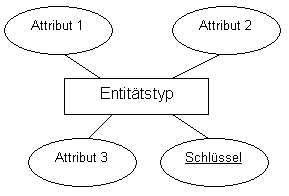
\includegraphics[scale=1,keepaspectratio=true]{./Bilder/entitaet.png}
 % entitaet.png: 0x0 pixel, 0dpi, nanxnan cm, bb=
 \caption{Darstellung von Entitätstypen und zugehörigen Attributen}
 \label{fig:entitaet}
\end{figure}
 \subsubsection{Schlüssel}
  \begin{mydef}
    Der \textbf{Primärschlüssel} ist eine minimale Kombination von Attributen, durch deren Werte jede Entität eindeutig identifiziert wird. Die Werte dürfen sich während der Existenz der Entität nicht ändern. Wir unterscheiden zwischen:
    \begin{description}
      \item[einfacher Schlüssel] der Primärschlüssel besteht aus einem Attribut
      \item[zusammengesetzter Schlüssel] der Primärschlüssel besteht aus mehreren Attributen, jedes Attributbezeichnet man als Teilschlüsselattribut.
      \item[künstlicher Schlüssel] das Attribut wurde zusätzlich für den Entitätstyp erschaffen (ID,..).
    \end{description}
 \end{mydef}
$\dashrightarrow$ Im Entity-Relationship-Modell werden die Attribute des Schlüssels unterstrichen.
 
 \subsubsection{Beziehungen}
 \begin{mydef}
  Eine \textbf{Beziehung} verbindet eine oder mehrere Entitäten miteinander. Assoziieren stets zwei Entitäten miteinander, so spricht man von \textit{binärer Beziehung}.  Ein \textbf{Beziehungstyp} umfasst alle Beziehungen, die gleichartig und wechselseitig zwischen zwei Entitätstypen bestehen. Ein Beziehungstyp kann Attribute besitzen. 
 \end{mydef}
$\dashrightarrow$ Für die Darstellung von Beziehungstypen nutzt man das Rautensymbol und notiert darin den Beziehungstyp als Name.
\begin{figure}[h]
 \centering
 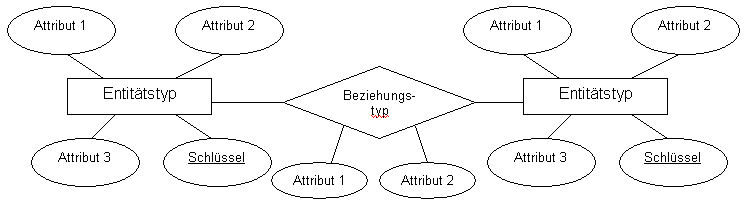
\includegraphics[width=1\textwidth]{./Bilder/beziehungen.png}
 % beziehungen.png: 0x0 pixel, 0dpi, nanxnan cm, bb=
 \caption{Darstellung von Beziehungstypen und zugehörigen Attributen}
 \label{fig:beziehungen}
\end{figure}

 \subsubsection{Kardinalität und Optionalität}
 \begin{mydef}
  Die \textbf{Kardinalität} zwischen dem Entitätstyp 1 und dem Entitätstyp 2 gibt an, wie viele Entitäten des Entitätstyps 2 höchstens mit einer Entität des Entitätstyps 1 in Beziehung stehen.
 \end{mydef}
 Für die Datenstrukturierung interessieren nicht die genauen Zahlen, sondern nur die durch die Chen-Notation vorgegebenen Typen
 \begin{itemize}
  \item höchstens eine Entität (1),
  \item mehrere Entitäten (n oder m).
 \end{itemize}
 Da der Beziehungstyp wechselseitig ist, wird die Kardinalität durch zwei Angaben vollständig beschrieben.\\
 In der \textit{modifizierten Chen-Notation} lässt sich die \textbf{Optionalität} durch Hinzufügen eines $c$s \textit{(von engl. can)} darstellen.

 \section{Das Relationenmodell}
 \subsection{Notation}
 Die Notation erfolgt folgendermaßen:
  \begin{center}
    Entitätstyp(\underline{Primärschlüssel}, Nichtschlüsselattribut, \textuparrow Fremdschlüssel)
  \end{center}
  
 \subsection{Regeln für die Transformation des ERM in das 
relationale Datenbankmodell}
\begin{enumerate}
  \item Entitätstypen:
  \begin{itemize}
    \item Jeder Entitätstyp wird in ein eigenes Relationsschema (Tabelle) abgebildet.
    \item Schlüssel werden kenntlich gemacht.
  \end{itemize}
  \item Beziehungstypen:
  \begin{itemize}
    \item Jeder Beziehungstyp wird in ein eigenes Relationsschema abgebildet. 
    \item Die Primärschlüssel der beiden beteiligten Entitätstypen werden zusätzliche Attributen des Relationsschemas. 
    \item Der (Teil-)Schlüssel des Relationsschemas bildet sich in Abhängigkeit von der Kardinalität wie folgt: 
  \end{itemize}
\end{enumerate}
    {%
\newcommand{\mc}[3]{\multicolumn{#1}{#2}{#3}}
\begin{center}
\begin{tabularx}{\columnwidth}{|c|X|} \hline
\textbf{Typ} & \mc{1}{c|}{\textbf{Schlüssel}}\\ \hline \hline
1:1 & einer der Primärschlüssel der beiden beteiligten Entitätstypen\\ \hline
1:n & der Primärschlüssel des zweiten Entitätstyps (also der "n-Entität")\\ \hline
n:m & beide Primärschlüssel der beteiligten Entitätstypen in neuem Relationstyp \\ \hline
    \end{tabularx}
    \end{center}
}%

\section{MySQL}
\lstset{language=SQL}
\subsection{SQL-Operationen}
SQL (Structured Query Language) ist eine Programmiersprache der 4. Generation und \textit{die} Sprache zum Aufbau, zur Verwaltung und zur Abfrage von relationalen Datenbanken. Sie wurde von IBM im Rahmen eines Forschungsprojektes entwickelt und 1987 international standardisiert. (Fast) alle Datenbanksysteme arbeiten mit dieser Sprache.

\subsubsection{Befehle zur Definition von Tabellen und anderer Datenstrukturen}       

\begin{lstlisting}[caption=Databank erzeugen]
 CREATE DATABASE "datenbankname";
\end{lstlisting}

\begin{lstlisting}[caption=Tabelle erzeugen]
CREATE TABLE "Tabellen_Name"
("Spalte 1" "Datentyp_Spalte_1",
"Spalte 2" "Datentyp_Spalte_2",
... );
\end{lstlisting}

\begin{lstlisting}[caption=Tabelle löschen]
DROP TABLE "Tabellen_Name";
\end{lstlisting}

\begin{lstlisting}[caption=Tabellenaufbau ändern]
ALTER TABLE "Tabellen_Name"
[Alter Spezifikation];
\end{lstlisting}
[Alter Spezifikation] hängt von der Art der gewünschten Änderung ab. Für die oben aufgeführten Anwendungszwecke lauten die entsprechenden Anweisungen:
\begin{itemize}
  \item Spalte hinzufügen: ADD ``Spalte 1'' ``Datentyp für Spalte 1''
  \item Spalte löschen: DROP ``Spalte 1''
  \item Spaltenname ändern: CHANGE ``alter Spaltenname'' ``neuer Spaltenname'' ``Datentyp für neuen Spaltennamen''
  \item Datentyp einer Spalte ändern: MODIFY ``Spalte 1`` ''neuer Datentyp``
\end{itemize}

\subsubsection{Befehle zur Datenmanipulation und Datenabfrage}      
tbd
\begin{lstlisting}[caption=Tabelle abfragen]
SELECT {spalten | *}
  FROM tabelle [alias] [tabelle [alias]] ...
    [WHERE {bedingung | unterabfrage}]
      [GROUP BY spalten]
      [ORDER BY spalten [ASC | DESC]...];
\end{lstlisting}
Die Syntax lässt sich wie folgt verstehen:
\begin{center}
\begin{tabularx}{\columnwidth}{|c|X|} \hline
\textbf{Klausel} & \textbf{Erläuterung}\\ \hline
SELECT & \textbf{Wähle} die Werte aus der/den Spalte(n)\\ \hline
FROM &  ... \textbf{aus} der Tabelle bzw. den Tabellen ...\\ \hline
WHERE & ... \textbf{wobei} die Bedingung(en) erfüllt sein soll(en) ...\\ \hline
GROUP BY & ... und \textbf{gruppiere} die Ausgabe von allen Zeilen mit gleichem Attributwert zu einer einzigen ...\\ \hline
ORDER BY [ASC/DESC] & ... und \textbf{sortiere} nach den Spalten \textit{[auf- bzw. absteigend]}. \\ \hline
\end{tabularx}
\end{center}
Bedingungen lassen sich mit \textbf{AND}, \textbf{OR} und \textbf{NOT} verknüpfen. Das \textbf{Sternsymbol} steht als Wildcard für eine beliebige Folge von Zeichen. Soll ein einzelnes Zeichen ausgeblendet werden, so benutzt man das Fragezeichen als Joker.
\begin{center}
\begin{tabularx}{\columnwidth}{|c|X|} \hline
\textbf{Operator} & \textbf{Erklärung}\\ \hline
$=$ $<$ $<=$ $>=$ $>$ $<>$ & vergleicht ein Attributwert mit einem anderen bzw. Konstante auf
Gleichheit, kleiner als, kleiner gleich, größer gleich, größer, Ungleichheit \\ \hline
BETWEEN ... AND ... &  vergleicht, ob der Attributwert zwischen zwei Grenzen liegt\\ \hline
IN (..., ..., ...) & vergleicht, ob der Attributwertein Element der Menge ist\\ \hline
LIKE & vergleich von Zeichenketten anhand von Ähnlichkeitsoperatoren mit Unterscheidung auf Groß- und Kleinschreibung: \newline
\%: Platzhalter für beliebiege Zeichen \newline
\_: Platzhalter für ein Zeichen\\ \hline
IS (NOT) NULL & prüft, ob ein Attributwert (nicht) undefiniert ist \\ \hline
\end{tabularx}
\end{center}
\vspace{5ex}
\begin{lstlisting}[caption=Inner Join]
SELECT "Spaltenliste"
  FROM "Haupttabelle"
  INNER JOIN "NebenTabelle" ON "Bedingung2;
\end{lstlisting}
Der Join gibt im Gegensatz zum Select an genau zwei Tabellen nicht das kartesisches Produkt ($A \times B$) der beiden Tabellen aus.

 \subsection{Datentypen in MySql (Auswahl)}
 \begin{description}
  \item [char(n)] Zeichenkette mit $n$ Zeichen $n \leq 255$, Rest wird mit 0en aufgefüllt
  \item [varchar(n)] Zeichenkette von variabler Länge $m \leq 255$
  \item [text] Text mit maximaler Länge: $65.535$
  \item [date] Datum
  \item [year] Yahr
  \item [integer(n)] Ganzzahl
  \item [float(m)] Gleitkommazahl, $m$ Nachkommastellen
  \item [decimal(n,m)] Festkommazahl n Stellen und m Nach dem Komma
  \item [boolean] Wahrheitswert
 \end{description}


 
 
 
\appendix  
\part{Anhang}
%\bibliographystyle{alpha}
\bibliographystyle{alphadin}
\bibliography{Bibl}
\begingroup
\printindex 
\endgroup
\section{Gruppen, Ringe, Körper} \label{subsec:GRK}
   Entnommen aus dem Propädeutikum der Universität Leipzig.
   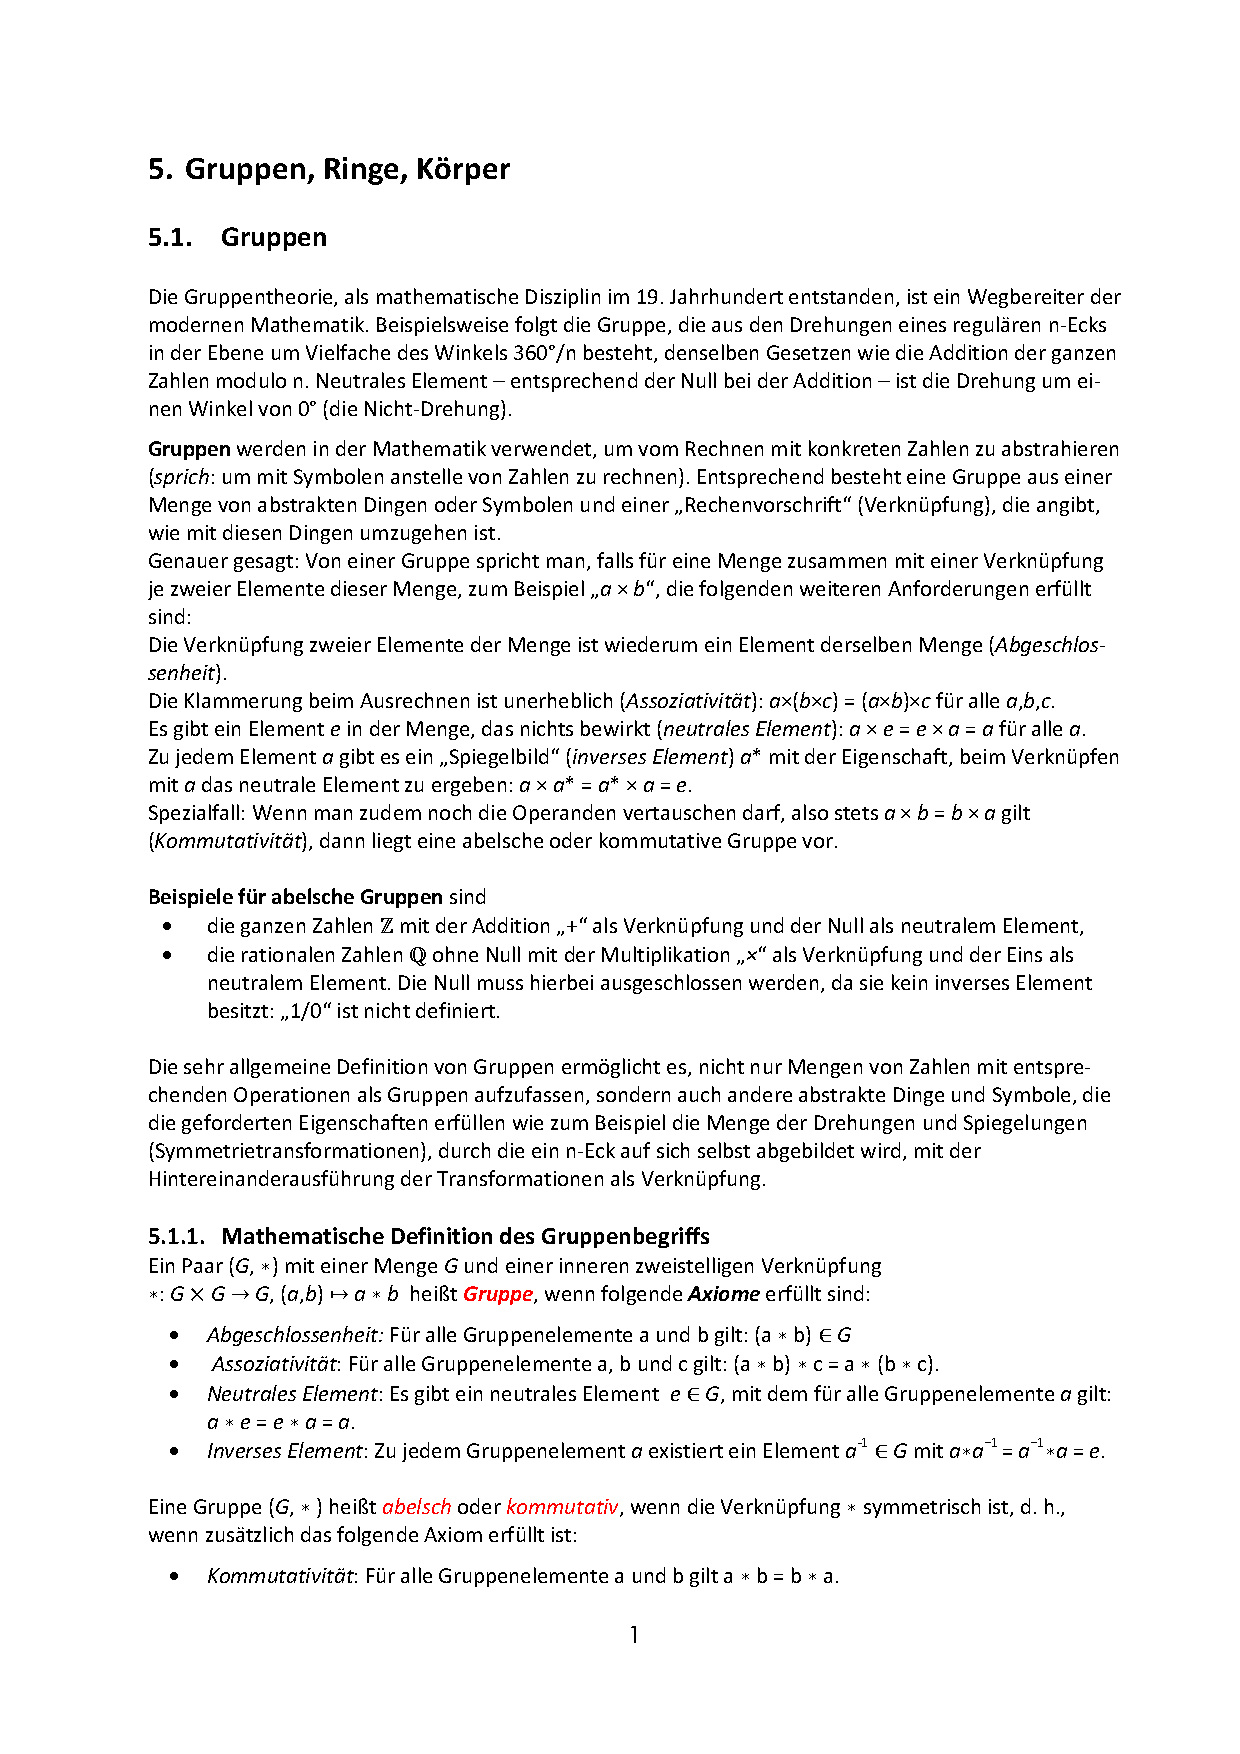
\includepdf[pages={1-6}]{gruppenringekoerper.pdf}

   
\end{document}